\documentclass[11pt,openany]{report}
\usepackage[a4paper,margin=1in]{geometry}
\usepackage{mathptmx}
\usepackage[T1]{fontenc}
\usepackage{amsmath,amssymb}
\usepackage{graphicx}
\usepackage{booktabs}
\usepackage{array}
\usepackage{longtable}
\usepackage{multicol}
\usepackage{float}
\usepackage{tikz}
\usepackage{xcolor}
\usepackage{setspace}
\usepackage{caption}
\usepackage{hyperref}
\usetikzlibrary{shapes.geometric,arrows.meta,positioning,fit,backgrounds,calc,decorations.pathreplacing}

\hypersetup{
  colorlinks=true,
  linkcolor=black,
  citecolor=black,
  urlcolor=blue!45!black,
  pdftitle={GlandersWatch: A Chained Multi-Level Machine Learning Framework for Population-Level Glanders Risk Prediction},
  pdfauthor={Yuvraj Singh},
  pdfsubject={B.Tech Project Report, International Institute of Information Technology, Bhubaneswar}
}

\graphicspath{{../figures/}}
\captionsetup{font=small,labelfont=bf,skip=6pt}
\setlength{\parskip}{0.35em}
\setlength{\parindent}{0pt}
\setlength{\emergencystretch}{1.5em}
% single spacing, as in the department template

% Section numbering follows the department template: sections are "1.", "2." within
% each chapter (counter resets per chapter) and subsections are "1.1", "1.2".
\renewcommand{\thesection}{\arabic{section}.}
\renewcommand{\thesubsection}{\arabic{section}.\arabic{subsection}}

% chapter-based numbering for floats and equations
\counterwithin{figure}{chapter}
\counterwithin{table}{chapter}
\renewcommand{\thefigure}{\thechapter.\arabic{figure}}
\renewcommand{\thetable}{\thechapter.\arabic{table}}

\input{diagstyles.tex}
\begin{document}
% The department template numbers continuously in arabic from the Certificate page,
% with the title page carrying no number, so Abstract falls on page 4.
\pagenumbering{arabic}
\setcounter{page}{0}

% ============================== TITLE PAGE ==============================
% Layout measured from the department template: title flush with the top margin,
% the emblem centred below the supervisor block at 3.2 cm, department block at foot.
\begin{titlepage}
\thispagestyle{empty}
\begin{center}

{\huge\bfseries GlandersWatch: A Chained\\[6pt]
Multi-Level Machine Learning\\[6pt]
Framework for Population-Level\\[6pt]
Glanders Risk Prediction\par}

\vspace{1.0cm}

{\large Project Report Submitted\par}
\vspace{0.5em}
{\normalsize in partial fulfillment of the requirements for the award of the\par}

\vspace{0.9cm}
{\large\bfseries Bachelor of Technology\par}
\vspace{0.3em}
{\large in\par}
\vspace{0.25em}
{\large\bfseries Computer Engineering\par}

\vspace{1.15cm}
{\large by\par}
\vspace{0.35em}
{\large\bfseries Yuvraj Singh \quad XXXXXXXXX\par}

\vspace{1.05cm}
{\large Under the supervision of\par}
\vspace{0.35em}
{\large\bfseries Dr. [Supervisor Name]\par}

\vspace{1.25cm}

\includegraphics[width=3.19cm]{iiit_logo.png}\par

\vfill

{\normalsize Department of Computer Science and Engineering\par}
\vspace{0.35em}
{\normalsize International Institute of Information Technology, Bhubaneswar\par}
\vspace{0.35em}
{\normalsize November 2026\par}

\vspace*{0.85cm}

\end{center}
\end{titlepage}

% ============================== CERTIFICATE ==============================
\newpage
\thispagestyle{empty}
\noindent\underline{\textbf{Certificate}}

\vspace{0.9cm}
\noindent
{\sloppy
This is to certify that the report entitled ``GlandersWatch: A Chained Multi-Level Machine
Learning Framework for Population-Level Glanders Risk Prediction'' submitted by
Yuvraj Singh (XXXXXXXXX) to International Institute of Information Technology, Bhubaneswar is a
record of bonafide project work under my supervision, and the report is submitted for the
evaluation of the BTech Degree Final-Semester Project.\par}

\vspace{1.6cm}
\noindent
\underline{(Supervisor)}\\[0.25em]
Dr. [Supervisor Name]

% ============================== DECLARATION ==============================
\newpage
\thispagestyle{empty}
\noindent\underline{\textbf{Declaration}}

\vspace{0.9cm}
\noindent
I certify that

\begin{enumerate}
  \item The work contained in the report has been done by myself under the general supervision of
        my supervisor.
  \item The work has not been submitted to any other Institute for any degree or diploma.
  \item I have followed the guidelines provided by the Institute in writing the report.
  \item I have conformed to the norms and guidelines given in the Ethical Code of Conduct of the
        Institute.
  \item Whenever I have used materials (data, theoretical analysis, and text) from other sources,
        I have given due credit to them by citing them in the text of the report and giving their
        details in the references.
  \item Whenever I have quoted written materials from other sources, I have put them under
        quotation marks and given due credit to the sources by citing them and giving required
        details in the references.
\end{enumerate}

\vspace{1.6cm}
\noindent
Yuvraj Singh\\
XXXXXXXXX

% ============================== ACKNOWLEDGMENTS ==============================
\newpage
\thispagestyle{empty}
\noindent\underline{\textbf{Acknowledgments}}

\vspace{0.9cm}
\noindent
I would like to express my sincere gratitude to my respected supervisor, Dr. [Supervisor Name], for the
invaluable guidance, support and encouragement given throughout this project. Their insights and
expertise were instrumental in shaping this work and helped me overcome numerous challenges. I am
also thankful to the faculty and staff of the Department of Computer Science and Engineering,
International Institute of Information Technology, Bhubaneswar, for providing the resources and a
conducive learning environment. Finally, I would like to thank my family and friends for their
unwavering support and understanding during the course of this project.

\vspace{1.6cm}
\noindent
Yuvraj Singh\\
XXXXXXXXX

% ============================== ABSTRACT ==============================
\newpage
\pagestyle{plain}
\noindent\underline{\textbf{Abstract}}
\addcontentsline{toc}{chapter}{Abstract}

\vspace{0.7cm}
\noindent
Glanders is a bacterial zoonosis of equids caused by \textit{Burkholderia mallei}. It is
notifiable, frequently fatal, and remains endemic in parts of Africa, Asia and South America.
Indian surveillance between 2019 and 2023 identified 728 seropositive equids across 138
districts, with strong geographic concentration. The published machine learning literature on
this disease is confined to laboratory identification of the organism by spectroscopic methods.
No population-level geographic risk model has been reported.

\vspace{0.5em}
\noindent
This project develops such a model. Four public datasets that had not previously been applied to
glanders are combined into a country-year panel: a text-mined occurrence corpus from Europe PMC,
FAOSTAT livestock stocks, World Bank development indicators and NASA POWER reanalysis
climatology. The panel contains 3,078 country-year observations across 162 equine-holding
countries for the years 2005 to 2023, with 172 positive labels and 44 engineered features.

\vspace{0.5em}
\noindent
Six model families are trained under three validation schemes, and a three-stage chained pipeline
is evaluated in which animal population is forecast before occurrence is predicted. On a forward
temporal holdout the strongest model reaches a precision-recall AUC of 0.554 against a base rate
of 0.056, an approximately ten-fold lift, with an expected calibration error of 0.016.
Performance falls to 0.304 under leave-country-out validation, which is the honest estimate for
an unseen country. Chaining produces no measurable gain in discrimination. An ablation shows that
climate covariates transfer poorly across countries, and the model performs least well in
low-income regions. The dominant limitation is that the label reflects documented activity rather
than true incidence, so the model largely learns which countries report disease. Reporting effort
is identified as the principal confounder for future work.

\vspace{0.7em}
\noindent
\textbf{Keywords:} Glanders, \textit{Burkholderia mallei}, Zoonosis, Risk Prediction, Class
Imbalance, Gradient Boosting, Probability Calibration, SHAP, Text Mining, Animal Health
Surveillance.

% ============================== CONTENTS ==============================
\newpage
\pagestyle{plain}
\noindent\underline{\textbf{Contents}}
\vspace{0.55cm}

% \tableofcontents would insert its own chapter-style heading and a page break;
% \@starttoc typesets the entries alone, under the heading above.
\makeatletter
\@starttoc{toc}
\makeatother

% =====================================================================
\chapter{Introduction}
\label{ch:intro}
% =====================================================================

\section{Background}

Glanders is a contagious and potentially fatal disease of horses, donkeys and mules caused by
the Gram-negative bacterium \textit{Burkholderia mallei}. The organism has no environmental
reservoir. Infection persists through transmission among equids, and asymptomatic carriers can
remain infectious for extended periods. Human infection is rare but carries a high case fatality
rate, and occurs through occupational contact with infected animals. The disease is notifiable
to the World Organisation for Animal Health and is classified as a potential bioterrorism agent.

The economic significance of glanders is concentrated in low and middle income countries, where
equids remain essential to transport, construction, agriculture and brick manufacture. India
recorded 5.44 lakh equids in the 2019 Livestock Census, a large proportion held by households
that depend on the animals for daily income. For such households the loss of a working animal is
a direct loss of livelihood, which makes early warning valuable even where mass treatment is not
feasible.

Surveillance data indicate that the disease is neither rare nor geographically contained. A
national programme screening 158,798 equid serum samples from 391 districts between 2019 and
2023 identified 728 seropositive animals in 138 districts, with roughly sixty per cent of
positives reported from Uttar Pradesh. Historical surveillance covering 2006 to 2018 reported
1,145 positive equids among 128,404 sera tested. These figures describe a persistent, spatially
structured problem rather than isolated outbreaks.

\section{Problem Definition}

The operational question facing a district veterinary officer is not whether glanders exists in
the country, but whether it is likely to appear in a given area in the coming year. Answering it
requires combining several kinds of evidence: the history of the disease in and around the area,
the size of the susceptible population, and the environmental conditions that permit
transmission.

Surveillance systems report what has already happened. Forecasting systems exist for several
livestock diseases but not for glanders. The problem addressed here is therefore the construction
and honest evaluation of a population-level risk model for glanders using only publicly
accessible data.

The problem has four parts.

\begin{enumerate}
  \item \textbf{Data assembly.} No single public source records glanders occurrence completely.
        Occurrence must be reconstructed from the literature and joined to population and
        environmental covariates at a common geographic and temporal resolution.
  \item \textbf{Label construction.} The outcome is rare, which makes naive accuracy useless and
        requires an explicit treatment of what a negative observation means.
  \item \textbf{Model selection under distribution shift.} A model fitted on some countries must
        be evaluated on countries it has never seen, because that is the deployment condition.
  \item \textbf{Threshold economics.} A probability is not an alert. The operating point must be
        chosen so that the volume of warnings is defensible relative to the events caught.
\end{enumerate}

\section{Objectives}

The objectives of the project are:

\begin{enumerate}
  \item To assemble a country-year panel for glanders from public sources not previously applied
        to this disease, covering animal history, animal population and environment.
  \item To engineer and select features using statistical evidence rather than assumption, and to
        document which evidence was used and why.
  \item To train and compare six model families under three validation schemes, with the harder
        scheme governing model selection.
  \item To design and evaluate a chained pipeline in which animal population is forecast as an
        intermediate step.
  \item To produce calibrated probabilities and an alert operating curve, so that the output can
        support a warning decision rather than only a ranking.
  \item To report limitations and negative results explicitly, including any component that failed
        to improve performance.
\end{enumerate}

\section{Scope and Limitations}

The study is scoped to country-year resolution. District-level modelling, which the original
project proposal envisaged for India, is not attempted here because the required district-level
covariates could not be assembled from public sources within the project period.

The model is a population-level risk tool. It does not diagnose an individual animal and is not
a substitute for laboratory confirmation or clinical examination.

Three limitations are stated at the outset because they shape every result that follows. First,
the label is derived from published reports, so a negative observation may indicate absence of
disease or absence of reporting. Second, occurrence is reconstructed by an automated extractor
that has not been validated against a hand-annotated reference set. Third, with 172 positive
observations the statistical uncertainty on every headline metric is substantial, and this is
quantified rather than hidden.

\section{Organisation of the Report}

Chapter~\ref{ch:lit} reviews the epidemiological and machine learning literature and identifies
the gap addressed here. Chapter~\ref{ch:method} describes the data, the panel construction, the
feature engineering and the modelling approach. Chapter~\ref{ch:impl} covers the implementation,
including the software architecture and both computational pipelines.
Chapter~\ref{ch:results} presents and discusses the results. Chapter~\ref{ch:concl} concludes and
sets out future work.

% =====================================================================
\chapter{Literature Review and Gap Analysis}
\label{ch:lit}
% =====================================================================

\section{Glanders Epidemiology and Burden}

Glanders is reviewed in the veterinary literature as a neglected zoonosis with high case
fatality and a genuine occupational risk to handlers \cite{khan2013,kanani2026}. A recent
systematic review and meta-analysis consolidates seroprevalence estimates across published
studies and identifies management practice and animal movement as the dominant epidemiological
drivers \cite{purnama2026}. Regional reviews document continued circulation in Brazil
\cite{mota2022}, and the disease remains endemic or repeatedly reported across parts of Africa,
Asia and the Middle East.

The consistent finding across this literature is that glanders persists where equid populations
are large, where animals move frequently, and where surveillance is weak. The first two
conditions are measurable from public data. The third affects whether the disease is visible at
all, and is therefore a confounder rather than a covariate.

\section{Surveillance in India}

Indian surveillance provides the strongest evidence base for the disease. Malik et al. described
the emergence and re-emergence of glanders in India through outbreaks reported between 2006 and
2011 \cite{malik2012}. Singha et al. reported serological surveillance and clinical investigation
of indigenous equines for the period 2015 to 2018 \cite{singha2020}. More recently, the national
programme covering 2019 to 2023 screened samples from 391 districts and produced a prevalence
estimate together with a risk analysis \cite{singha2026}.

These studies establish where glanders occurs, which districts carry the burden, and which
animal-level factors are associated with seropositivity. None constructs a predictive model, and
none uses population or reanalysis covariates as predictors.

\section{Geographic and Spatiotemporal Risk Analysis}

Descriptive spatial analysis of glanders has been reported. Fonseca-Rodr\'iguez et al. applied
spatiotemporal cluster detection to Brazilian glanders data \cite{fonseca2019}. More broadly,
species distribution and ecological niche models have been compared as tools for livestock and
disease epidemics \cite{hollings2017}.

This body of work is descriptive. Cluster detection identifies where cases have already
concentrated. It does not forecast which cells will be positive in a future period, and that
distinction matters for an early warning application, where the value lies in anticipating
rather than confirming.

\section{Machine Learning for Animal Disease Risk}

Predictive modelling of animal disease risk is established for avian influenza. Kane et al.
compared ARIMA and random forest models for the prediction of H5N1 outbreaks \cite{kane2014}.
Walsh et al. used machine learning to target active surveillance for avian influenza viruses
\cite{walsh2019}. Yoo et al. developed dynamic farm-level risk prediction for highly pathogenic
avian influenza in the Republic of Korea \cite{yoo2022}, and Alshatti et al. produced a risk
prediction model for outbreaks in Kuwait \cite{alshatti2026}.

This literature supplies the methodological template used here: assemble occurrence, population
and environmental covariates at a common spatial unit, fit tree-based ensembles, and evaluate on
held-out periods. The template has been applied to influenza, and not to glanders.

\section{Machine Learning and Glanders}

The only machine learning work specific to \textit{Burkholderia mallei} that could be located is
spectroscopic identification of the organism. Moawad et al. developed a Raman spectroscopic assay
in which learned models classify spectra to identify \textit{B. mallei} and related species
\cite{moawad2019}. St\"ockel et al. reported Raman spectroscopic detection and identification of
\textit{B. mallei} and \textit{B. pseudomallei} \cite{stoeckel2015}.

Both are laboratory diagnostic problems. Neither addresses the geographic or temporal
distribution of the disease, and neither produces a risk estimate for a population.

\section{Text Mining for Disease Event Extraction}

Using published literature as a structured source of occurrence data has precedent in epidemic
intelligence. Collier surveyed web-based epidemic intelligence and the role of text mining within
it \cite{collier2012}, and Lejeune et al. described multilingual event extraction for epidemic
detection \cite{lejeune2015}.

The present work applies sentence-level event extraction not as a supplementary signal but as the
primary source of the label, for the pragmatic reason that official outbreak records are
incomplete for many countries. The consequence, that the label inherits both the strengths and
the reporting biases of the literature, is analysed rather than assumed away.

\section{Prior Art Audit}

To test the novelty claim rather than assert it, a reproducible set of queries was run against
Europe PMC. Each row of Table~\ref{tab:novelty} is a query count, and the full query strings and
retrieved titles are retained alongside the project code.

\begin{table}[htbp]
\centering
\caption{Europe PMC hit counts for combinations of glanders with each data source and method used
in this study.}
\label{tab:novelty}
\small
\begin{tabular}{@{}lc@{}}
\toprule
\textbf{Query} & \textbf{Hits} \\
\midrule
glanders (baseline corpus) & 6674 \\
glanders + machine learning & 75 \\
glanders + tree ensembles & 40 \\
glanders + forecasting & 139 \\
glanders + FAOSTAT & 7 \\
glanders + NASA POWER & 0 \\
glanders + World Bank indicators & 22 \\
glanders + equine population denominator & 54 \\
glanders + Europe PMC text mining & 378 \\
glanders + chained/stacked models & 36 \\
glanders + random forest (risk context) & 8 \\
glanders + niche / distribution model & 62 \\
glanders + remote sensing / reanalysis & 10 \\
glanders + spatio-temporal clustering & 463 \\
glanders + gradient boosting & 4 \\
\bottomrule
\end{tabular}
\end{table}

The decisive cells are the query pairing glanders with NASA POWER, which returns zero records,
and the pairing with gradient boosting, which returns four, none of which is a glanders risk
model. The nearest prior work is descriptive cluster detection in Brazil and a risk-factor
analysis of the Indian serosurvey.

\section{Research Gap}

The literature reviewed above divides into three disjoint groups. Epidemiological studies
describe where glanders occurs. Machine learning studies of \textit{B. mallei} classify laboratory
spectra. Veterinary risk models exist but are built for influenza. No study joins an occurrence
corpus, a livestock census, development indicators and reanalysis climatology into a single panel
for glanders, and none evaluates a calibrated predictive model on that panel.

That gap defines the contribution of this project.

% =====================================================================
\chapter{Methodology}
\label{ch:method}
% =====================================================================

\section{Data Sources}

Four publicly accessible sources are used. None had previously been applied to glanders risk
modelling, and each contributes a distinct kind of evidence.

\begin{table}[htbp]
\centering
\caption{Data sources and their role in the panel.}
\label{tab:sources}
\small
\begin{tabular}{@{}p{2.9cm}p{2.7cm}p{4.3cm}p{3.4cm}@{}}
\toprule
\textbf{Source} & \textbf{Role} & \textbf{Content} & \textbf{Coverage} \\
\midrule
Europe PMC & Animal history & Occurrence events extracted from abstracts & 6,674 records, 263 events \\
FAOSTAT & Animal population & Stocks of horses, asses, mules, camels, cattle, sheep and goats & 68,449 records, 1961--2023 \\
World Bank & Socio-economic context & Ten development indicators and country centroids & 217 countries, 2000--2024 \\
NASA POWER & Environment & Temperature, precipitation, humidity and wind & Six measures, 211 centroids, 2005--2024 \\
\bottomrule
\end{tabular}
\end{table}

Figure~\ref{fig:coverage} shows the distribution of the extracted occurrence events by year and
by country. The volume of recorded activity rises after 2015, which reflects growth in open
access veterinary publishing as much as any change in disease incidence. This is one reason the
label is treated as documented activity throughout.

\begin{figure}[htbp]
\centering
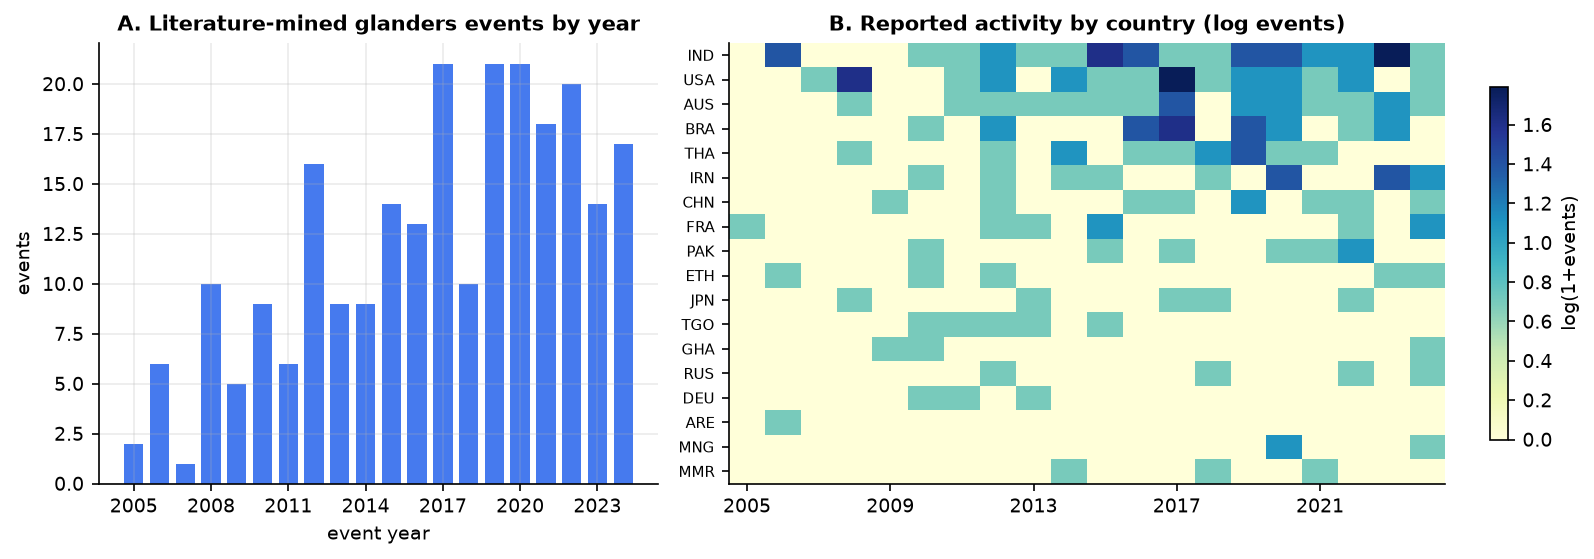
\includegraphics[width=\textwidth]{fig01_dataset_coverage.png}
\caption{Occurrence events extracted from Europe PMC. Panel A gives the annual count. Panel B
gives the distribution across the most frequently reporting countries on a logarithmic scale.}
\label{fig:coverage}
\end{figure}

\section{Panel Construction}

All four sources are keyed on ISO 3166 alpha-3 country code and calendar year, so they join
without ambiguity once names are reconciled. FAOSTAT is streamed from the 32\,MB compressed bulk
archive, which expands to approximately 545\,MB, and filtered to the seven stock series of
interest rather than loaded into memory.

Country names are matched to ISO-3 through \texttt{pycountry} with explicit overrides for
non-standard forms such as ``T\"urkiye'', ``Viet Nam'' and ``C\^ote d'Ivoire''. World Bank
regional and global aggregates are excluded by requiring a three-character ISO code, which
prevents rows such as ``World'' or ``South Asia'' from entering the panel as if they were
countries.

The full grid contains 6,700 country-year rows across 268 countries for 2000
to 2024. For modelling, three restrictions are applied: only equine-holding countries are
retained, defined as a maximum equid stock of at least one thousand animals; only the years 2005
to 2023 are used; and only rows with an observable next-year label are kept. The resulting matrix
has 3,078 rows, 44 features and 172 positive labels.

\section{Preprocessing}

\subsection{Duplicate Removal}

Extracted events are de-duplicated on the composite key of country, year and source record
identifier. Without this step a single paper reporting several cases would contribute multiple
counts and inflate the occurrence signal.

\subsection{Missing Values}

Missing numeric values are imputed with the column median, and every column that required
imputation keeps a binary missing-indicator feature so that absence is represented rather than
silently filled. Imputation is fitted inside the training pipeline, so the test period cannot
influence imputed values. Missingness is low: 0.00\% in the FAOSTAT block, 1.68\% in the
World Bank block, 2.19\% in the climate block, and 0.99\% overall, with no column
exceeding 5.8\%.

\subsection{Treatment of Absence}

A country-year is assigned a negative label only after the country passes the equine-stock
filter. This prevents a country with no recorded equids from contributing an uninformative
negative observation, and ensures that a blank is never read as proof that disease was absent.

\section{Label Definition}

The prediction target is binary: whether a glanders occurrence was documented in country $i$
during year $t+1$. Occurrence is extracted from Europe PMC by matching, within a single sentence,
a country name from a curated gazetteer and a term from an occurrence lexicon containing
\emph{outbreak}, \emph{case}, \emph{detected}, \emph{seropositive} and \emph{surveillance}. When
both are present, an event is recorded for the year stated in the sentence, or the publication
year where no year is stated.

Because the label depends on publication it is termed \emph{documented activity} throughout. A
negative value may indicate either the absence of disease or the absence of a report, and the
model is therefore interpreted as a predictor of surveillance-observable activity.

\section{Feature Engineering}

Four groups of features are constructed, all using information available at time $t$ or earlier.

\begin{table}[htbp]
\centering
\caption{Feature groups, sizes and rationale.}
\label{tab:features}
\small
\begin{tabular}{@{}p{2.7cm}cp{9.6cm}@{}}
\toprule
\textbf{Group} & \textbf{Count} & \textbf{Content and rationale} \\
\midrule
Disease history & 7 & Occurrence in the two prior years, a five-year running total, years since the last event, and contemporaneous world and regional activity shares. The disease persists in an area once introduced. \\
Animal population & 14 & Log equid and total livestock stocks, equid share of farm animals, equid density, one- and three-year growth, and the seven species counts. A larger susceptible population offers more opportunity for detection. \\
Climate & 10 & Mean, maximum and minimum temperature, precipitation total and coefficient of variation, relative humidity and wind, each paired with an anomaly computed against the country's own expanding mean. The anomaly separates unusual conditions from latitude. \\
Socio-geography & 11 & Income band, agricultural land share, agricultural value added, livestock production index, GDP per capita, rural share, internet penetration, fertiliser intensity, life expectancy, population and density. These largely proxy surveillance capacity. \\
\bottomrule
\end{tabular}
\end{table}

Three derived features require definition. Equid share is the sum of horses, asses and mules
divided by total farm animals. Livestock units apply metabolic weights, with cattle and camels at
0.8 and small ruminants at 0.1, so that one number expresses grazing pressure across species.
Years since the last event uses the value 99 to denote no recorded event within the panel window.

\section{Feature Selection}

Selection proceeded in two stages. First, columns with no measurable association with the label
were removed. Mutual information and Spearman correlation were computed for every numeric
feature, and columns with mutual information below 0.002 and absolute correlation below 0.02 were
discarded. Second, redundancy was addressed. One member of each pair with absolute correlation at
or above 0.90 was removed, and a column that was exactly the sum of three others was dropped
because a tree model can construct that sum itself.

No linear projection or principal component analysis was applied. With 44 features and
3,078 rows the binding constraint proved to be signal rather than dimensionality. This is
supported by the ablation in Section~\ref{sec:ablation}, which shows that reduced feature sets
generalise better across countries than the full set.

The selection criterion is itself examined in Section~\ref{sec:selection}, where marginal and
conditional importance are compared.

\section{Models}

Six model families are compared. The set spans the range from additive to fully interactive, and
includes a deliberately simple reference.

\begin{table}[htbp]
\centering
\caption{Model families and the hyperparameters selected by tuning.}
\label{tab:models}
\small
\begin{tabular}{@{}p{2.6cm}p{2.3cm}p{9.2cm}@{}}
\toprule
\textbf{Model} & \textbf{Family} & \textbf{Selected configuration} \\
\midrule
\textbf{Logistic regression} & linear & Additive model with balanced class weights; the reference baseline.\par\vspace{2pt}{\footnotesize Tuned settings: $C=1.0$, $\ell_2$ penalty, balanced class weights} \\
\textbf{Decision tree} & tree & Single shallow tree; interpretable, and a low-variance check on ensemble gains.\par\vspace{2pt}{\footnotesize Tuned settings: depth 3, minimum leaf size 1, criterion entropy} \\
\textbf{Random forest} & bagged trees & Bagged trees over random subsets; variance control at small positive counts.\par\vspace{2pt}{\footnotesize Tuned settings: depth 6, minimum leaf size 1, features per split square root of the column count} \\
\textbf{Extra trees} & bagged trees & Bagged trees with randomised split thresholds; further decorrelation when positives are scarce.\par\vspace{2pt}{\footnotesize Tuned settings: depth 6, minimum leaf size 10, features per split 0.3} \\
\textbf{XGBoost} & boosted trees & Boosted trees with explicit regularisation.\par\vspace{2pt}{\footnotesize Tuned settings: depth 3, regularisation $\lambda=1.0$, minimum child weight 5} \\
\textbf{LightGBM} & boosted trees & Leaf-wise boosted trees; efficient comparison on wide tabular data.\par\vspace{2pt}{\footnotesize Tuned settings: leaves 15, minimum child samples 40, regularisation $\lambda=1.0$} \\
\bottomrule
\end{tabular}
\end{table}

Logistic regression provides an additive baseline with balanced class weights. A single decision
tree is included because shallow trees are interpretable by a non-specialist, and because the
performance gap between one tree and an ensemble is itself informative. Random forest and extra
trees are bagged ensembles, differing in the degree of randomisation applied to split selection.
XGBoost and LightGBM are boosted ensembles, differing in tree growth strategy \cite{chen2016,ke2017}.

Neural networks were excluded on evidential grounds. With 172 positive observations and
44 features, a network has far more parameters to estimate than it has positive examples
from which to learn, and would be expected to memorise the training period and fail on new data.

\section{Chained Pipeline}

The project proposal specified a multi-stage design. Three stages are implemented.

\begin{enumerate}
  \item \textbf{Population forecast.} Next-year log equid stock is predicted from the current
        year's covariates using ridge regression and histogram gradient boosting, evaluated by
        grouped cross-validation on country.
  \item \textbf{Occurrence.} The binary label is modelled with the forecast population appended as
        an additional feature, and compared against the same model without it.
  \item \textbf{Intensity.} Conditional on an event, log event count is modelled by a random forest
        regressor trained on positive observations only.
\end{enumerate}

The stages are combined into a hurdle model, in which expected event burden is the product of
event probability and conditional intensity.

\section{Evaluation Design}

Three validation schemes are reported, each answering a different question.

\begin{itemize}
  \item \textbf{Temporal holdout.} Training on 2005 to 2017 and testing on 2018 to 2023, with the
        test period never observed during fitting. This answers whether the model can be used in
        the following years.
  \item \textbf{Leave-country-out.} Five folds grouped by country, so every prediction is made for
        a country absent from training. This answers whether the model transfers to a new country,
        and it governs model selection because it is the harsher test and the closer
        approximation of deployment.
  \item \textbf{Repeated stratified cross-validation.} Five folds repeated three times, used as a
        stability check on the ranking metrics.
\end{itemize}

Precision-recall AUC is the primary metric. At 5.59\% prevalence, ROC-AUC is dominated by
the true-negative mass and overstates performance, a well-characterised property of imbalanced
problems \cite{saito2015,davis2006}. ROC-AUC is reported for comparability. Brier score and
expected calibration error are reported because an uncalibrated probability cannot support a
threshold-based alert \cite{niculescu2005,huang2020}. Precision, recall, specificity, F1 and the
Matthews correlation coefficient are computed at a threshold tuned on training data only, and
bootstrap percentile intervals with one thousand resamples quantify sampling uncertainty.

Grouped rather than random splitting is essential. A random row split would place the same country
in both training and test partitions, allowing the model to memorise country identity. Given the
geographic proxy effects described in Section~\ref{sec:selection}, this would inflate all reported
scores \cite{roberts2017}.

\section{Leakage Controls}

Six controls are applied.

\begin{enumerate}
  \item All features are built from year $t$ or earlier, and only the target columns use $t+1$.
  \item The split is chronological, so no future observation can enter training.
  \item Hyperparameters are tuned inside training folds using grouped cross-validation.
  \item Probability calibration is fitted on training folds only.
  \item The alert threshold is fixed on the training period and applied unchanged to test.
  \item Missing-indicator features and imputation values are generated inside the pipeline, so the
        test period cannot influence them.
\end{enumerate}

% =====================================================================
\chapter{Implementation}
\label{ch:impl}
% =====================================================================

\section{Software Architecture}

The project is implemented as a sequence of numbered scripts, each producing artefacts consumed
by the next. All intermediate outputs are cached, so any stage can be re-run without repeating
the stages before it.

\begin{table}[htbp]
\centering
\caption{Processing stages and their outputs.}
\label{tab:stages}
\small
\begin{tabular}{@{}p{4.3cm}p{4.0cm}p{6.2cm}@{}}
\toprule
\textbf{Script} & \textbf{Stage} & \textbf{Output} \\
\midrule
\texttt{00\_novelty\_audit} & Prior art audit & Query counts and retrieved titles \\
\texttt{01\_fetch\_data} & Ingestion & Europe PMC, World Bank and NASA POWER payloads \\
\texttt{01c\_extract\_faostat} & Ingestion & Seven FAOSTAT stock series \\
\texttt{02\_build\_panel} & Assembly & Panel, extracted events and audit block \\
\texttt{03\_train\_evaluate} & Modelling & Metrics, predictions and model comparison \\
\texttt{05\_dataset\_analysis} & Analysis & Association, redundancy and selection statistics \\
\texttt{04\_report}, \texttt{06\_analysis\_figures} & Reporting & Figures and summary tables \\
\texttt{09\_make\_full\_report} & Reporting & This document \\
\bottomrule
\end{tabular}
\end{table}

\section{Training Pipeline}

Figure~\ref{fig:trainflow} shows the training sequence. The chronological split is placed before
any model sees the data, so the test years cannot influence fitting, tuning or calibration.


\begin{figure}[htbp]
\centering
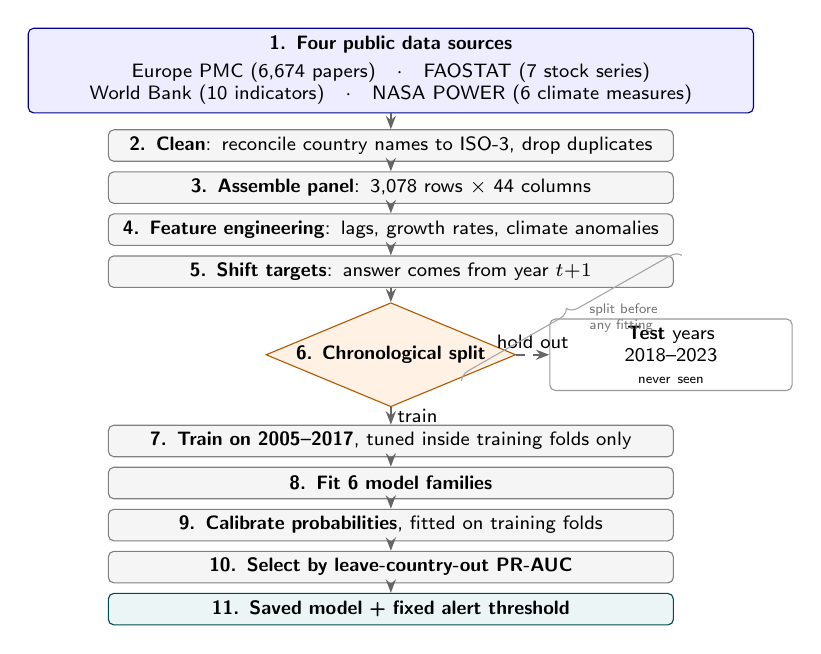
\begin{tikzpicture}[
  st/.style={rectangle,rounded corners=2pt,draw=black!50,fill=black!4,
             align=center,minimum height=0.40cm,text width=7.0cm,
             font=\scriptsize\sffamily,inner sep=2.5pt},
  srcbox/.style={rectangle,rounded corners=2pt,draw=blue!55!black,fill=blue!7,
             align=center,minimum height=0.80cm,text width=9.0cm,
             font=\scriptsize\sffamily,inner sep=3pt},
  dec/.style={diamond,draw=orange!70!black,fill=orange!10,aspect=2.4,
              align=center,font=\scriptsize\sffamily,inner sep=1pt},
  final/.style={rectangle,rounded corners=2pt,draw=teal!60!black,fill=teal!8,
             align=center,minimum height=0.40cm,text width=7.0cm,
             font=\scriptsize\sffamily,inner sep=2.5pt},
  testb/.style={rectangle,rounded corners=2pt,draw=black!40,fill=white,
             align=center,minimum height=0.52cm,text width=2.9cm,
             font=\scriptsize\sffamily,inner sep=2.5pt},
  fl/.style={-{Stealth[length=1.7mm]},thick,draw=black!60},
  step/.style={font=\scriptsize\sffamily\bfseries,text=black!45,anchor=east},
]

  \node[srcbox] (src) at (0,0)
    {\textbf{1. Four public data sources}\\[2pt]
     Europe PMC (6{,}674 papers)\quad$\cdot$\quad FAOSTAT (7 stock series)\\
     World Bank (10 indicators)\quad$\cdot$\quad NASA POWER (6 climate measures)};

  \node[st,below=0.20cm of src] (clean) {\textbf{2. Clean}: reconcile country names to ISO-3, drop duplicates};
  \node[st,below=0.12cm of clean] (panel) {\textbf{3. Assemble panel}: 3{,}078 rows $\times$ 44 columns};
  \node[st,below=0.12cm of panel] (feat) {\textbf{4. Feature engineering}: lags, growth rates, climate anomalies};
  \node[st,below=0.12cm of feat] (shift) {\textbf{5. Shift targets}: answer comes from year $t{+}1$};
  \node[dec,below=0.18cm of shift] (split) {\textbf{6. Chronological split}};

  % training branch (down)
  \node[st,below=0.22cm of split] (train) {\textbf{7. Train on 2005--2017}, tuned inside training folds only};
  \node[st,below=0.12cm of train] (fit) {\textbf{8. Fit 6 model families}};
  \node[st,below=0.12cm of fit] (cal) {\textbf{9. Calibrate probabilities}, fitted on training folds};
  \node[st,below=0.12cm of cal] (sel) {\textbf{10. Select by leave-country-out PR-AUC}};
  \node[final,below=0.12cm of sel] (saved) {\textbf{11. Saved model + fixed alert threshold}};

  % test branch (right)
  \node[testb,right=0.42cm of split] (test) {\textbf{Test} years\\2018--2023\\\tiny never seen};

  \draw[fl] (src) -- (clean);
  \draw[fl] (clean) -- (panel);
  \draw[fl] (panel) -- (feat);
  \draw[fl] (feat) -- (shift);
  \draw[fl] (shift) -- (split);
  \draw[fl] (split) -- node[font=\scriptsize\sffamily,right=1pt,inner sep=1pt] {train} (train);
  \draw[fl] (train) -- (fit);
  \draw[fl] (fit) -- (cal);
  \draw[fl] (cal) -- (sel);
  \draw[fl] (sel) -- (saved);
  \draw[fl,dashed] (split.east) -- node[font=\scriptsize\sffamily,above,inner sep=2pt] {hold out} (test.west);

  % brace showing where leakage protection sits
  \draw[decorate,decoration={brace,amplitude=4pt,mirror},black!35]
       ([xshift=0.10cm]shift.north east) -- ([xshift=0.10cm]split.south east)
       node[midway,right=3pt,font=\tiny\sffamily,text=black!55,align=left]
       {split before\\any fitting};
\end{tikzpicture}
\caption{Training pipeline. The chronological split sits before any model sees the
data, so the 2018--2023 years never influence training. Tuning and calibration both
happen strictly inside the training years.}
\label{fig:trainflow}
\end{figure}


\section{Evaluation Pipeline}

Figure~\ref{fig:evalflow} shows the evaluation sequence. One trained model is scored under three
schemes, each producing a different answer, and the resulting metrics are summarised with
uncertainty intervals.


\begin{figure}[htbp]
\centering
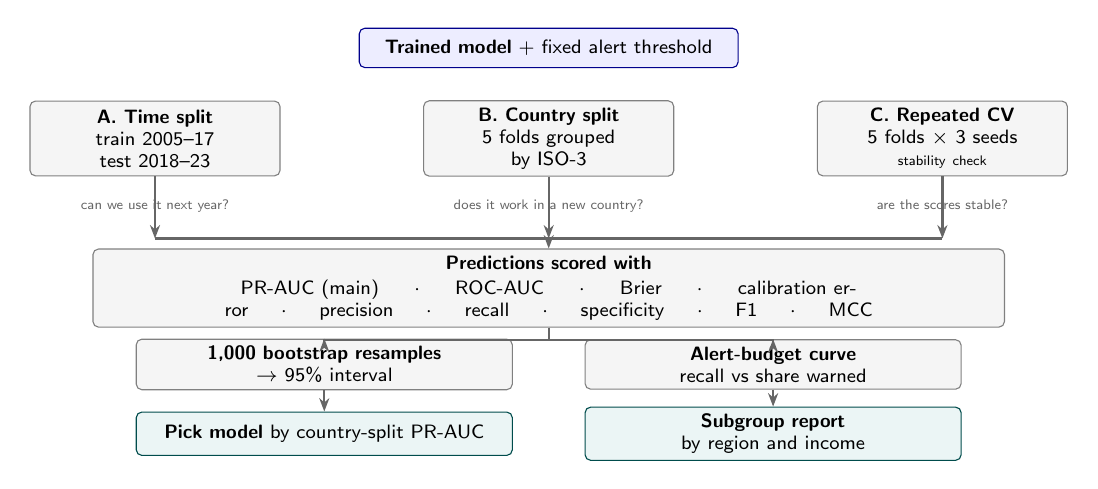
\begin{tikzpicture}[
  bx/.style={rectangle,rounded corners=2pt,draw=black!50,fill=black!4,
             align=center,font=\scriptsize\sffamily,inner sep=2.5pt},
  top/.style={rectangle,rounded corners=2pt,draw=blue!55!black,fill=blue!7,
             align=center,font=\scriptsize\sffamily,inner sep=3pt},
  fin/.style={rectangle,rounded corners=2pt,draw=teal!60!black,fill=teal!8,
             align=center,font=\scriptsize\sffamily,inner sep=2.5pt},
  fl/.style={-{Stealth[length=1.7mm]},thick,draw=black!60},
]

  \node[top,text width=4.6cm,minimum height=0.5cm] (m) at (0,0)
       {\textbf{Trained model} + fixed alert threshold};

  % three schemes
  \node[bx,text width=3.0cm,minimum height=0.95cm] (s1) at (-5.0,-1.15)
       {\textbf{A. Time split}\\train 2005--17\\test 2018--23};
  \node[bx,text width=3.0cm,minimum height=0.95cm] (s2) at (0,-1.15)
       {\textbf{B. Country split}\\5 folds grouped\\by ISO-3};
  \node[bx,text width=3.0cm,minimum height=0.95cm] (s3) at (5.0,-1.15)
       {\textbf{C. Repeated CV}\\5 folds $\times$ 3 seeds\\\tiny stability check};

  \node[font=\tiny\sffamily,text=black!60,anchor=north,text width=3.0cm,align=center] (q1)
       at (-5.0,-1.80) {can we use it next year?};
  \node[font=\tiny\sffamily,text=black!60,anchor=north,text width=3.0cm,align=center] (q2)
       at (0,-1.80) {does it work in a new country?};
  \node[font=\tiny\sffamily,text=black!60,anchor=north,text width=3.0cm,align=center] (q3)
       at (5.0,-1.80) {are the scores stable?};

  % collector rail
  \coordinate (railL) at (-5.0,-2.42);
  \coordinate (railR) at (5.0,-2.42);
  \draw[fl] (s1.south) -- (railL);
  \draw[fl] (s2.south) -- (0,-2.42);
  \draw[fl] (s3.south) -- (railR);
  \draw[thick,draw=black!60] (railL) -- (railR);

  \node[bx,text width=11.4cm,minimum height=0.78cm] (met) at (0,-3.05)
       {\textbf{Predictions scored with}\\[1pt]
        PR-AUC (main) $\;\cdot\;$ ROC-AUC $\;\cdot\;$ Brier $\;\cdot\;$ calibration error
        $\;\cdot\;$ precision $\;\cdot\;$ recall $\;\cdot\;$ specificity $\;\cdot\;$ F1
        $\;\cdot\;$ MCC};
  \draw[fl] (0,-2.42) -- (met.north);

  \node[bx,text width=4.6cm,minimum height=0.62cm] (boot) at (-2.85,-4.02)
       {\textbf{1{,}000 bootstrap resamples}\\$\rightarrow$ 95\% interval};
  \node[bx,text width=4.6cm,minimum height=0.62cm] (alert) at (2.85,-4.02)
       {\textbf{Alert-budget curve}\\recall vs share warned};

  \node[fin,text width=4.6cm,minimum height=0.55cm] (pick) at (-2.85,-4.90)
       {\textbf{Pick model} by country-split PR-AUC};
  \node[fin,text width=4.6cm,minimum height=0.55cm] (sub) at (2.85,-4.90)
       {\textbf{Subgroup report}\\by region and income};

  \draw[fl] (met.south) -- ++(0,-0.16) -| (boot.north);
  \draw[fl] (met.south) -- ++(0,-0.16) -| (alert.north);
  \draw[fl] (boot) -- (pick);
  \draw[fl] (alert) -- (sub);

\end{tikzpicture}
\caption{Evaluation pipeline. One trained model is scored three different ways, each
answering a different question, then reported with uncertainty intervals.}
\label{fig:evalflow}
\end{figure}


\section{Alert Engine Design}

The wider platform for which this model was built includes an alert service that converts a
predicted probability into a notification for registered owners and field workers. The rules
engine is shown in Figure~\ref{fig:alertarch}. Three rules govern whether a notification is
emitted. A threshold maps the calibrated probability to a risk level. A suppression rule decides
whether a message is warranted at all, based on state changes, cooldowns and a data-freshness
guard. A deduplication rule prevents the same alert being issued twice for the same area, period
and level.

\begin{figure}[htbp]
\centering
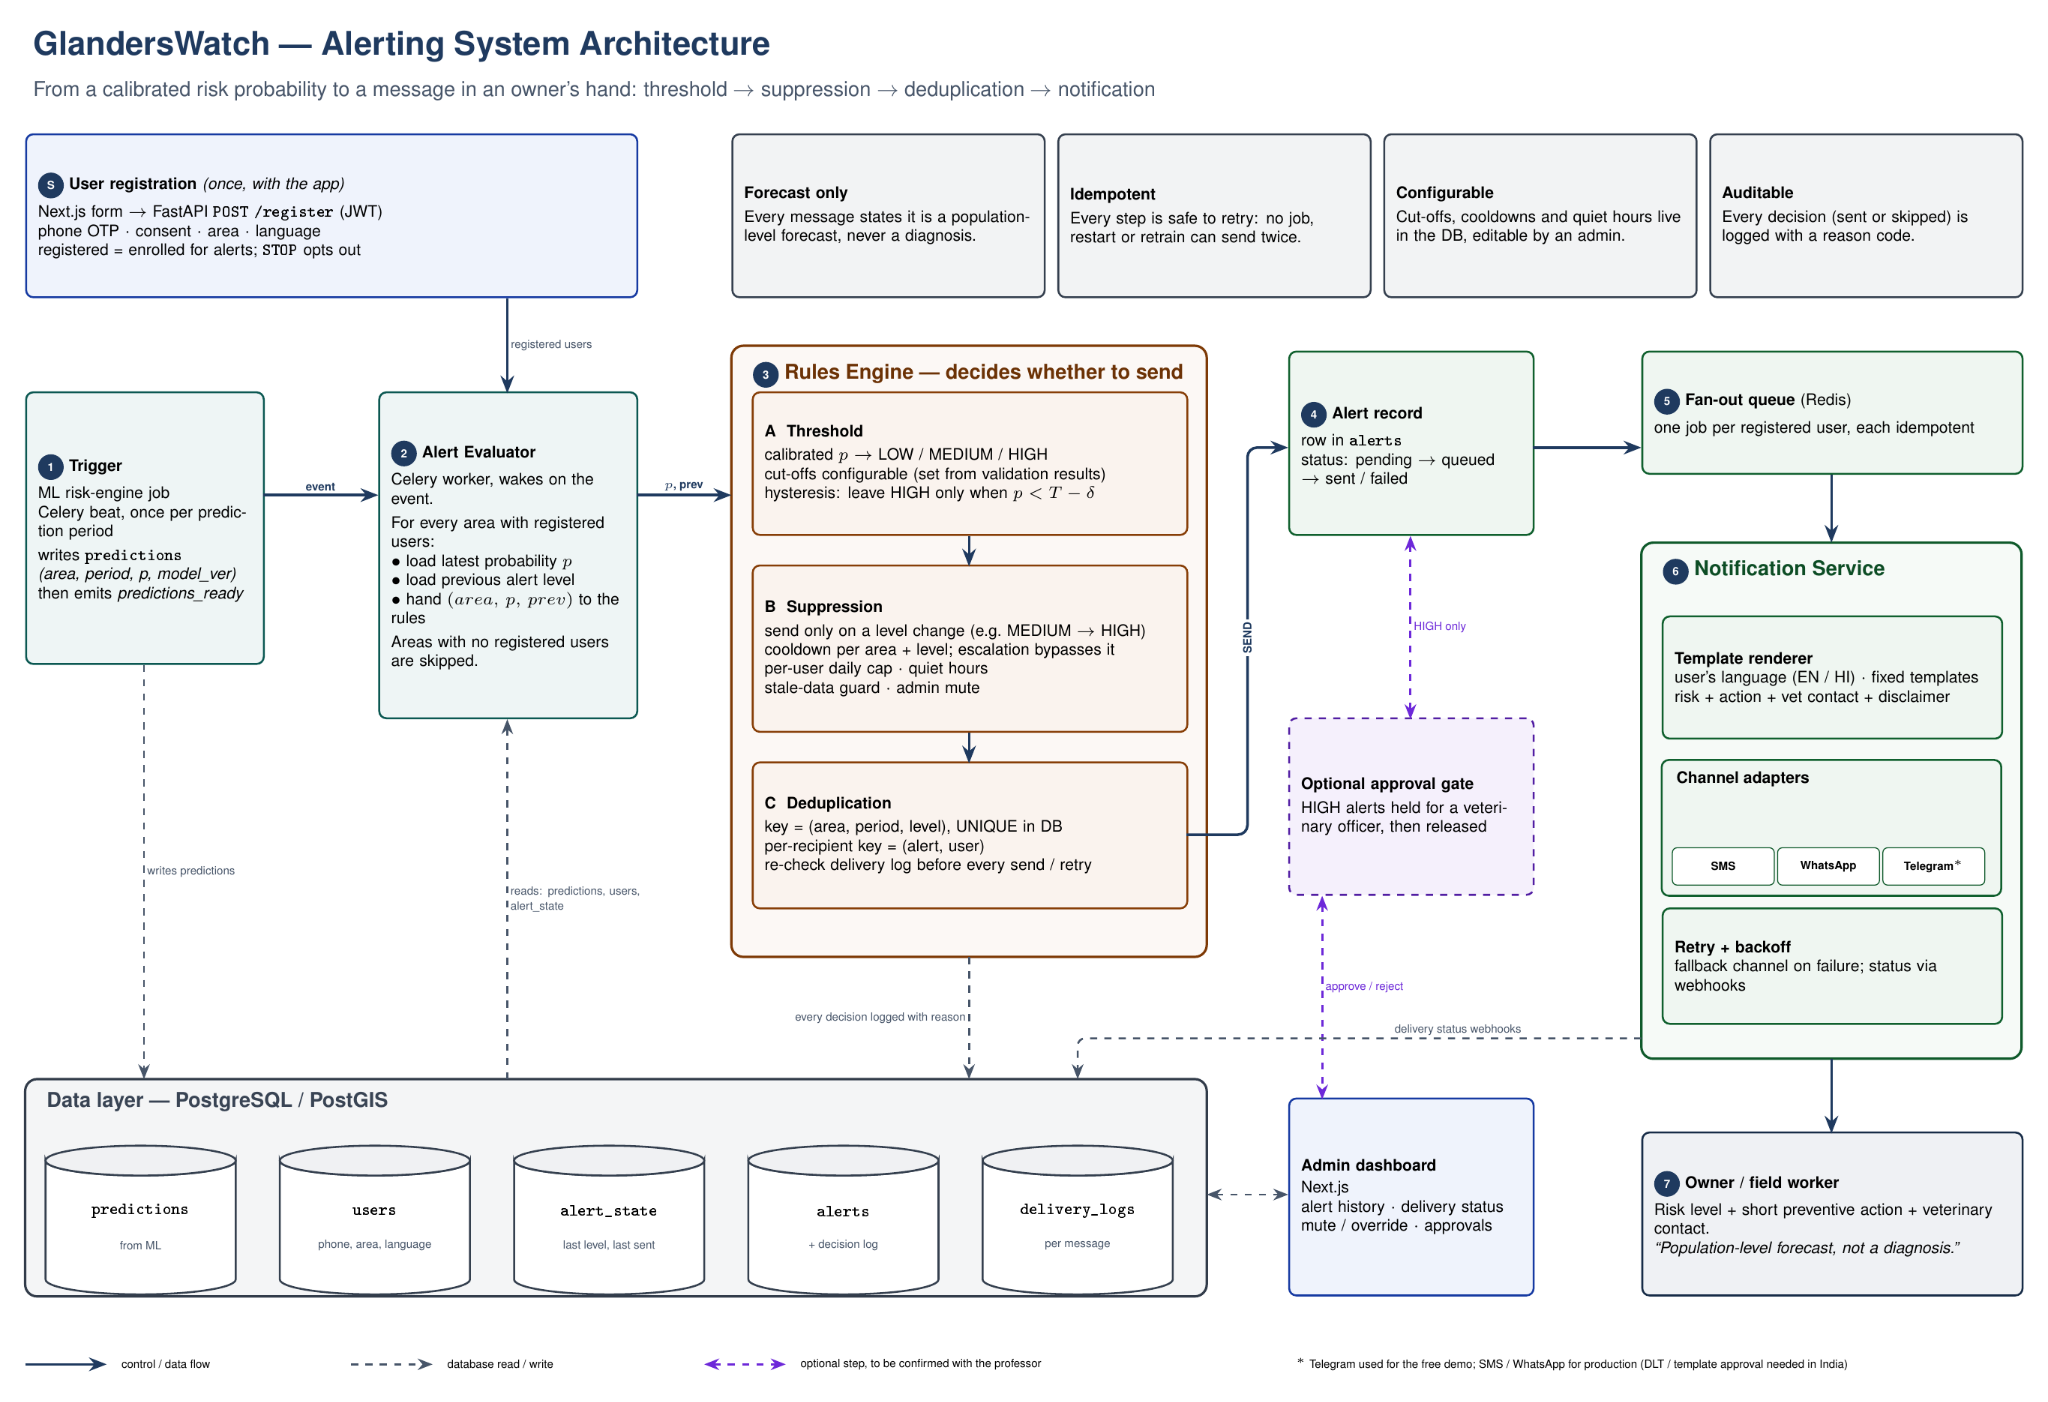
\includegraphics[width=\textwidth]{proposal_alert_architecture.png}
\caption{Architecture of the alert rules engine, reproduced from the project proposal. The
calibrated probability enters the threshold, suppression and deduplication rules before an alert
record is created and fanned out to notification channels.}
\label{fig:alertarch}
\end{figure}

The thresholds used by this engine are taken from the operating curve in
Section~\ref{sec:alerts} rather than from a default value. This is the practical link between the
modelling work reported here and the alerting behaviour of the platform.

\section{Reproducibility}

The full computation runs in approximately 4.5 minutes on a laptop processor without a
graphics accelerator, using an Apple M4 processor with 10 cores and 16 GB of unified memory. Per-family fitting time at the country-year level ranges
from 1.9 seconds for the decision tree to 50.7 seconds for LightGBM.

A single module-level seed constant governs model fitting, cross-validation splitting, bootstrap
resampling and SHAP sampling. Software versions are Python 3.12.13, scikit-learn 1.9.1, XGBoost 3.4.1, LightGBM 4.7.0, SHAP 0.54.1, NumPy 2.5.4, pandas 3.1.1, SciPy 1.18.1. Raw payloads are cached under
\texttt{data/raw} and the derived panel is written to \texttt{data/processed}, so every reported
number can be regenerated without re-downloading upstream sources.

One determinism caveat applies. Tree ensembles are seeded but not bitwise reproducible across
different thread counts, so parallel execution may change the final decimal of an ensemble score.

% =====================================================================
\chapter{Results and Discussion}
\label{ch:results}
% =====================================================================

\section{Dataset Characteristics}

The modelling matrix contains 3,078 country-year observations, of which 172 are
positive, a prevalence of 5.59\% and an imbalance ratio of 16.9 to one.
Table~\ref{tab:labels} summarises the distribution.

\begin{table}[htbp]
\centering
\caption{Characteristics of the label.}
\label{tab:labels}
\small
\begin{tabular}{@{}lr@{}}
\toprule
\textbf{Property} & \textbf{Value} \\
\midrule
Observations & 3,078 \\
Positives and negatives & 172 and 2,906 \\
Prevalence & 5.59\% \\
Imbalance ratio & 16.9 : 1 \\
Countries with at least one positive & 56 of 162 \\
Countries positive in two or more years & 30 \\
Share of positives in the top five countries & 35.5\% \\
\bottomrule
\end{tabular}
\end{table}

Three properties of this distribution matter. The imbalance rules out accuracy as a metric and
motivates precision-recall analysis. The temporal persistence of the label, with 30 of
56 positive countries recording positives in more than one year, justifies the use of
historical features. The geographic concentration of positives, with the top five countries
holding 35.5\% of them, provides the first indication that the label tracks reporting
capacity, since those countries operate reference laboratories.

Figure~\ref{fig:labels} presents the same information graphically, together with the regional
distribution of prevalence.

\begin{figure}[htbp]
\centering
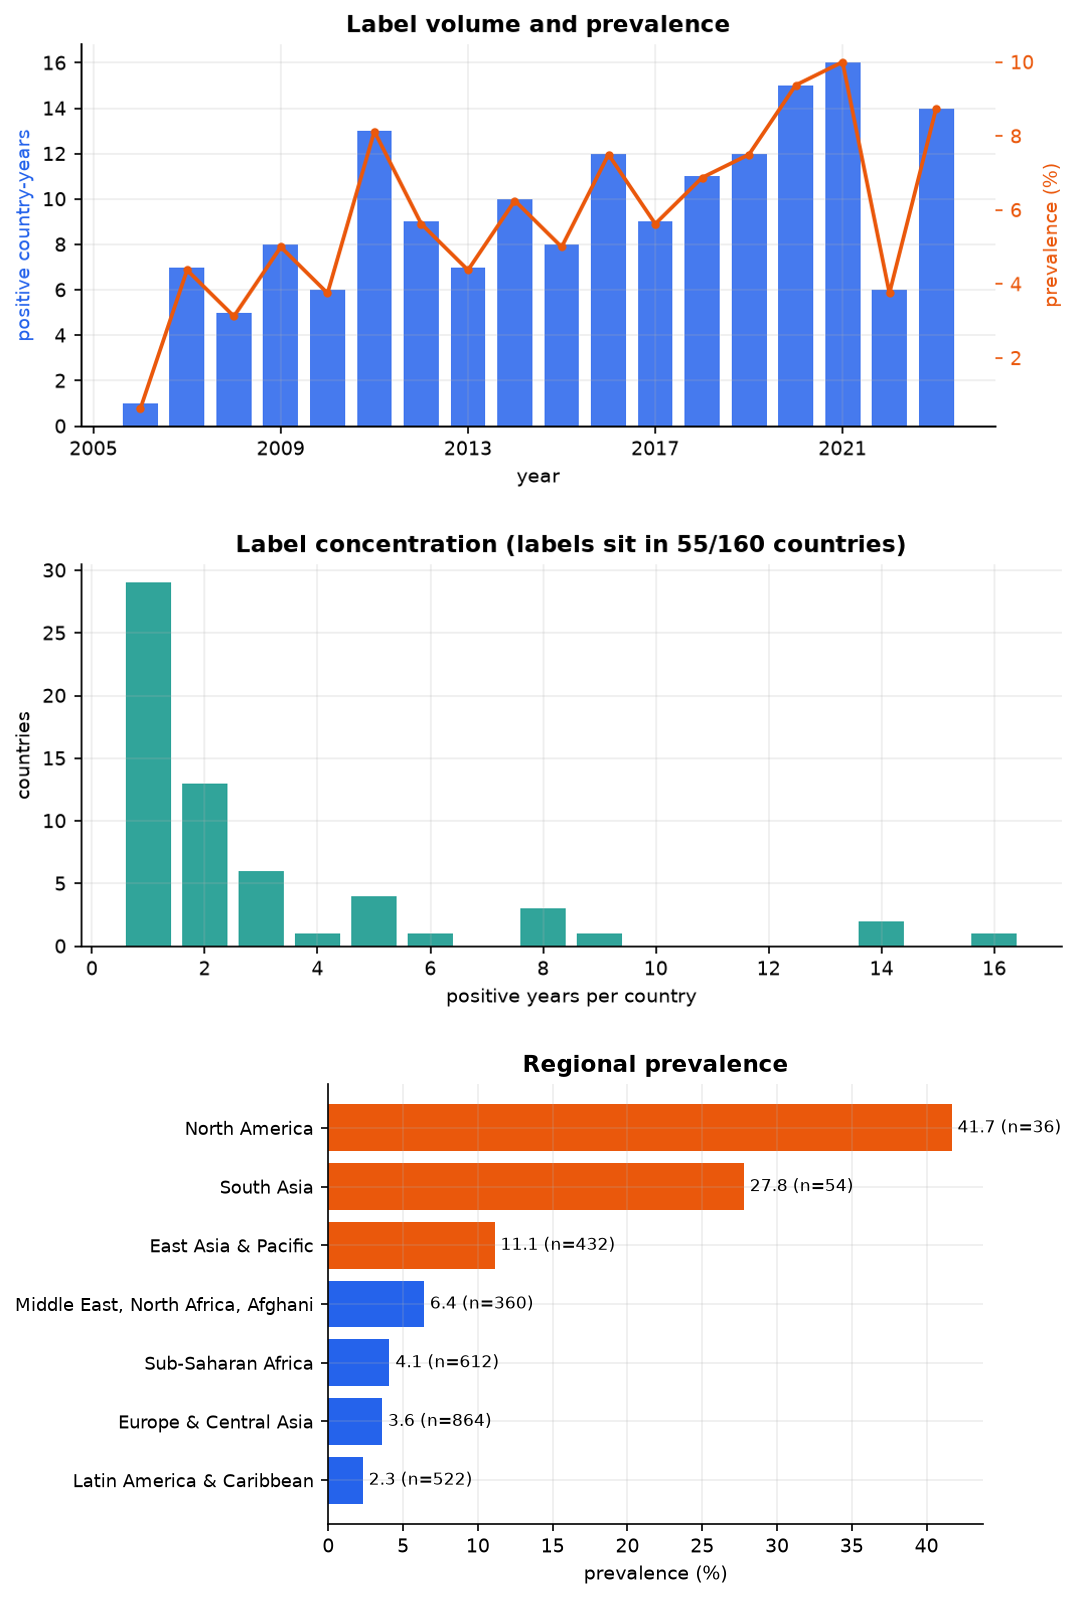
\includegraphics[width=\textwidth]{fig10_label_anatomy.png}
\caption{Label anatomy. Panel A gives annual positive counts with prevalence on the secondary
axis. Panel B gives the distribution of positive years per country. Panel C gives prevalence by
World Bank region.}
\label{fig:labels}
\end{figure}

\section{Statistical Association and Feature Selection}
\label{sec:selection}

Spearman correlation, mutual information and Cram\'er's $V$ were computed for every candidate
feature before any model was fitted. The strongest monotone association is
\texttt{years\_since\_last} at $\rho = -0.35$, negative because a longer interval since the
last recorded event implies lower risk. This is the most defensible epidemiological signal in the
panel. Among the categorical strata, region yields a Cram\'er's $V$ of 0.243, a small
association, and income band yields 0.047, which is negligible.

Redundancy is substantial. Variance inflation reaches 228 for \texttt{temp\_mean}, because
annual mean, minimum and maximum temperature are near-duplicates at country resolution.
Figure~\ref{fig:corr} shows the correlation structure of the highest-ranked features.

\begin{figure}[htbp]
\centering
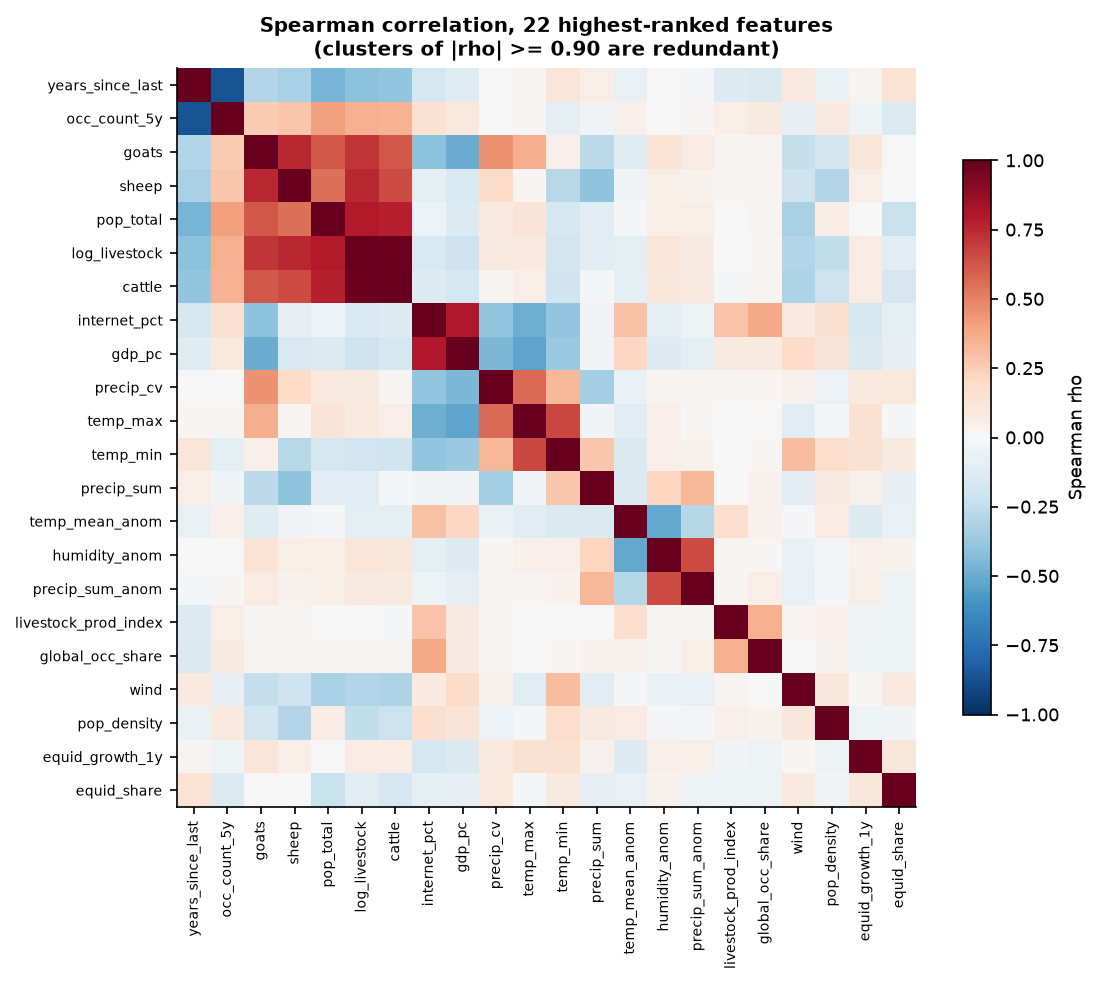
\includegraphics[width=0.76\textwidth]{fig11_correlation.png}
\caption{Spearman correlation matrix of the twenty-two highest-ranked features, hierarchically
ordered. Block structure indicates the collinear groups that motivated redundancy reduction.}
\label{fig:corr}
\end{figure}

The most consequential finding in this section concerns the choice of selection criterion.
Marginal association and conditional importance disagree almost completely. The rank correlation
between mutual information and SHAP attribution is -0.03, and only 5 of the ten
highest-ranked features are shared between the two orderings. \texttt{longitude} ranks first on
marginal correlation and approximately twentieth on conditional importance, because once
population and history are conditioned upon it carries little additional information. It
functions as a proxy for which part of the world a country occupies, and therefore for publishing
activity.

Figure~\ref{fig:views} shows the disagreement directly, and Table~\ref{tab:topfeat} gives the
ranked features with both sets of statistics. Ranking features by marginal association alone would
favour columns that track reporting practice rather than disease occurrence, so selection was
performed on conditional evidence instead.

\begin{figure}[htbp]
\centering
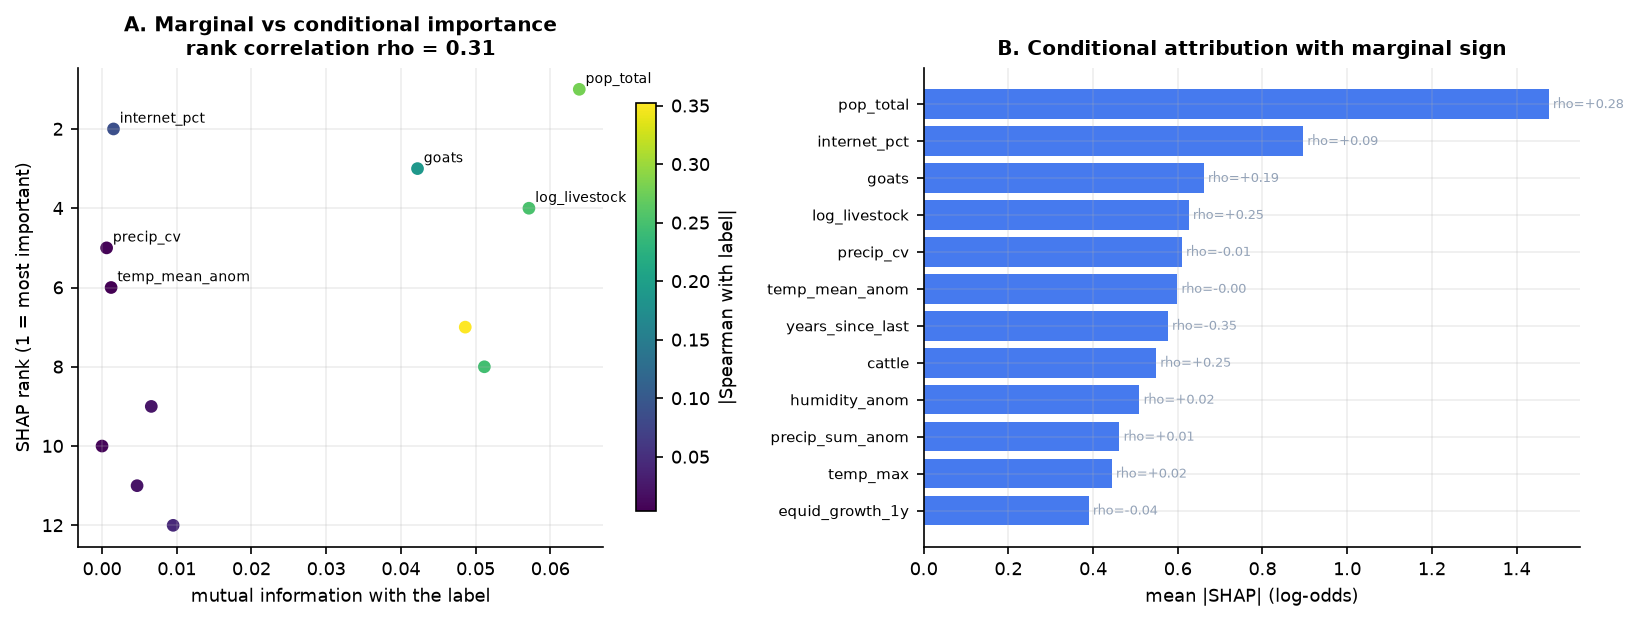
\includegraphics[width=\textwidth]{fig12_importance_views.png}
\caption{Marginal and conditional importance. Panel A plots mutual information against
conditional rank, and the absence of a downward trend is the disagreement quantified in the text.
Panel B gives the conditional ranking with the marginal association sign annotated.}
\label{fig:views}
\end{figure}

\begin{table}[htbp]
\centering
\caption{The eight highest-ranked features by mean absolute SHAP value, with marginal statistics
alongside for comparison.}
\label{tab:topfeat}
\small
\begin{tabular}{@{}rlrrrr@{}}
\toprule
\textbf{Rank} & \textbf{Feature} & \textbf{Mean $|$SHAP$|$} & \textbf{Spearman $\rho$} &
\textbf{Mutual info} & \textbf{VIF} \\
\midrule
1 & pop\_total & 1.144 & +0.28 & 0.0639 & 4 \\
2 & internet\_pct & 0.542 & +0.09 & 0.0015 & 5 \\
3 & temp\_mean\_anom & 0.469 & -0.00 & 0.0012 & 2 \\
4 & log\_livestock & 0.458 & +0.25 & 0.0571 & 3 \\
5 & humidity\_anom & 0.370 & +0.02 & 0.0066 & 2 \\
6 & years\_since\_last & 0.353 & -0.35 & 0.0486 & 2 \\
7 & wind & 0.346 & -0.08 & 0.0210 & 3 \\
8 & sheep & 0.344 & +0.20 & 0.0512 & 13 \\
\bottomrule
\end{tabular}
\end{table}

Figure~\ref{fig:shap} gives the global attribution for the full panel.

\begin{figure}[htbp]
\centering
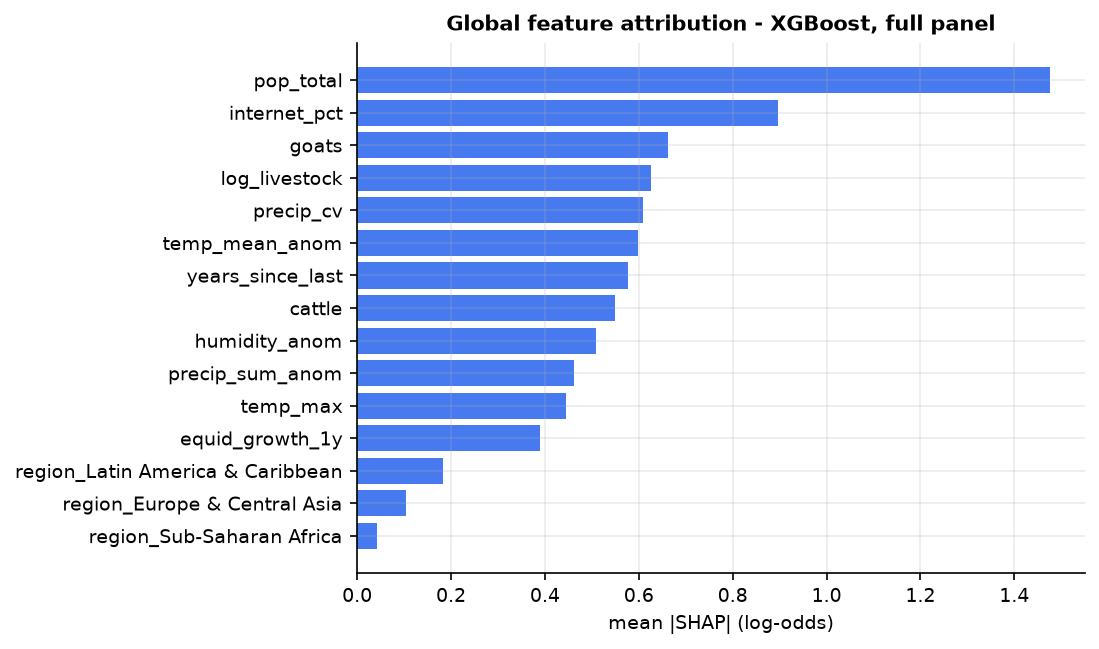
\includegraphics[width=0.72\textwidth]{fig06_shap.png}
\caption{Global feature attribution for XGBoost over the full panel, ordered by mean absolute SHAP
value. Population magnitude and reporting capacity dominate. Among biological drivers, recent
history and climate anomalies rank highest.}
\label{fig:shap}
\end{figure}

\section{Model Comparison}

Table~\ref{tab:level1} reports discrimination under all three schemes. The temporal holdout is the
realistic test and the leave-country-out result is the harder one.

\begin{table}[htbp]
\centering
\caption{Discrimination at the country-year level. Brackets give 95 per cent bootstrap intervals
on the temporal holdout.}
\label{tab:level1}
\small
\resizebox{\textwidth}{!}{%
\begin{tabular}{@{}lcccccccc@{}}
\toprule
\textbf{Model} & \textbf{PR-AUC} & \textbf{95\% CI} & \textbf{ROC-AUC} &
\textbf{PR-AUC} & \textbf{PR-AUC} & \textbf{Brier} & \textbf{Prec.} & \textbf{Rec.} \\
 & \textbf{(time)} & \textbf{on PR-AUC} & \textbf{(time)} & \textbf{(country)} &
\textbf{(rep.\ CV)} & & & \\
\midrule
Logistic regression & 0.454 & [0.34, 0.58] & 0.812 & 0.223 & 0.414 & 0.0547 & 0.25 / 0.57 \\
Decision tree & 0.389 & [0.29, 0.50] & 0.861 & 0.267 & 0.360 & 0.0602 & 0.49 / 0.53 \\
Random forest & 0.554 & [0.43, 0.66] & 0.870 & 0.304 & 0.476 & 0.0503 & 0.53 / 0.50 \\
Extra trees & 0.530 & [0.42, 0.64] & 0.854 & 0.363 & 0.476 & 0.0535 & 0.47 / 0.51 \\
XGBoost & 0.485 & [0.37, 0.60] & 0.844 & 0.281 & 0.423 & 0.0536 & 0.61 / 0.38 \\
LightGBM & 0.496 & [0.38, 0.61] & 0.841 & 0.339 & 0.397 & 0.0534 & 0.65 / 0.30 \\
\bottomrule
\end{tabular}}
\end{table}

Against a base rate of 5.59\%, the strongest temporal result of 0.554 represents an
approximately 10-fold lift. Every tree-based model exceeds the logistic baseline, and the
single decision tree is the weakest of the six, which indicates that the relationships are
interactive rather than additive.

The more important pattern is the systematic decline under leave-country-out validation. For
Random Forest the score falls from 0.554 to 0.304, and the decline exceeds the width of the
bootstrap interval for every family. This is the expected signature of learning country-specific
structure, and it is the estimate that should be quoted for deployment.

\begin{figure}[htbp]
\centering
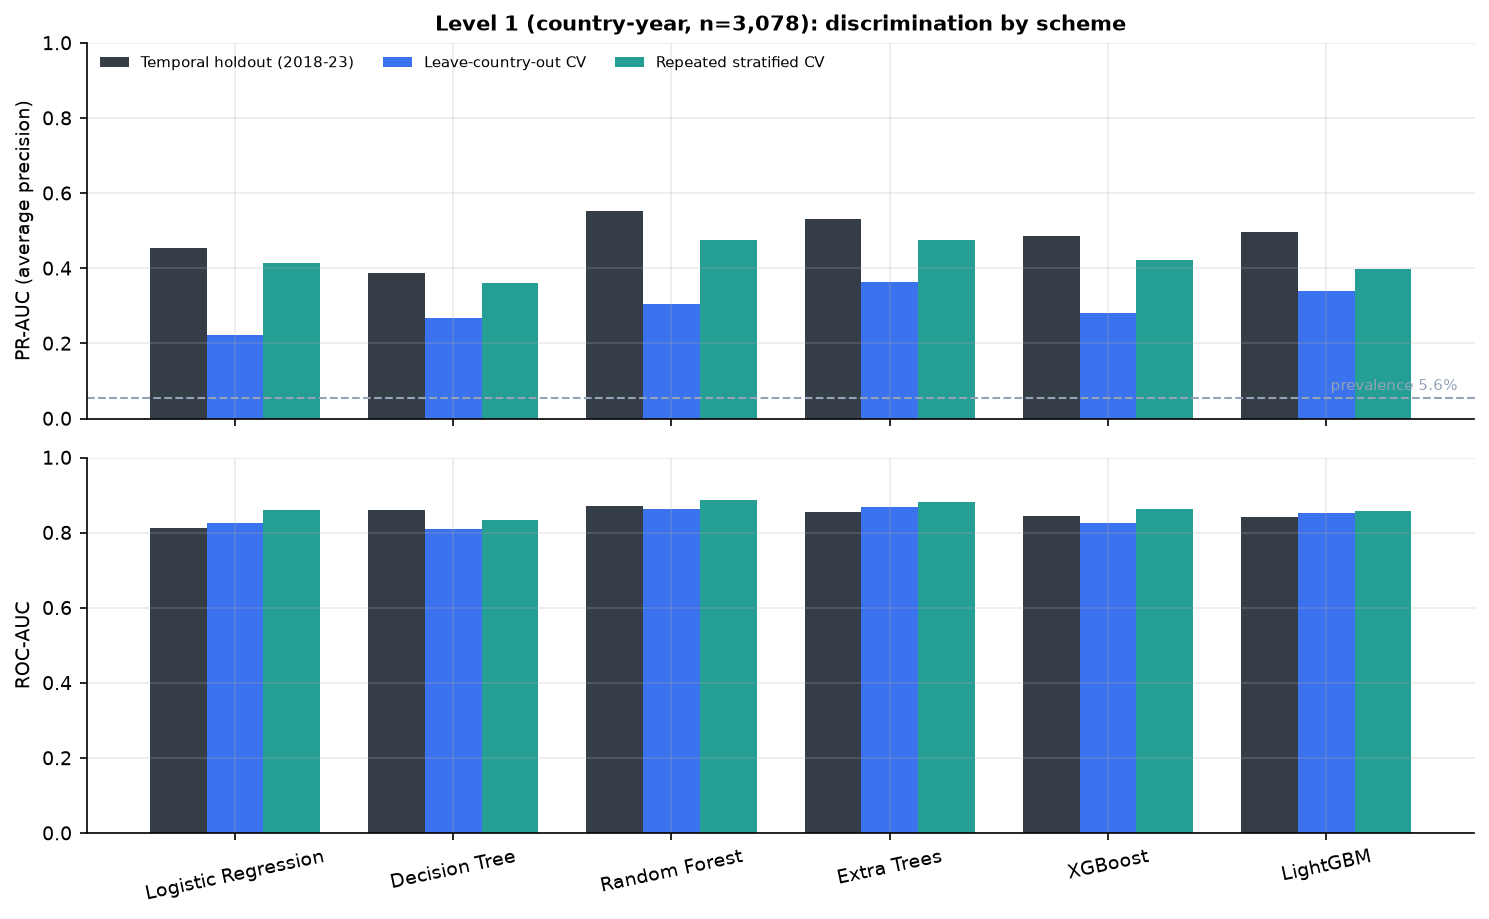
\includegraphics[width=\textwidth]{fig02_model_comparison.png}
\caption{Discrimination by model and validation scheme. The gap between repeated
cross-validation and leave-country-out validation is the cost of generalising to an unseen
country.}
\label{fig:comparison}
\end{figure}

Figure~\ref{fig:curves} shows the ROC and precision-recall curves for the temporal holdout. At
this prevalence the ROC curves compress into a narrow band while the precision-recall panel
separates the families.

\begin{figure}[htbp]
\centering
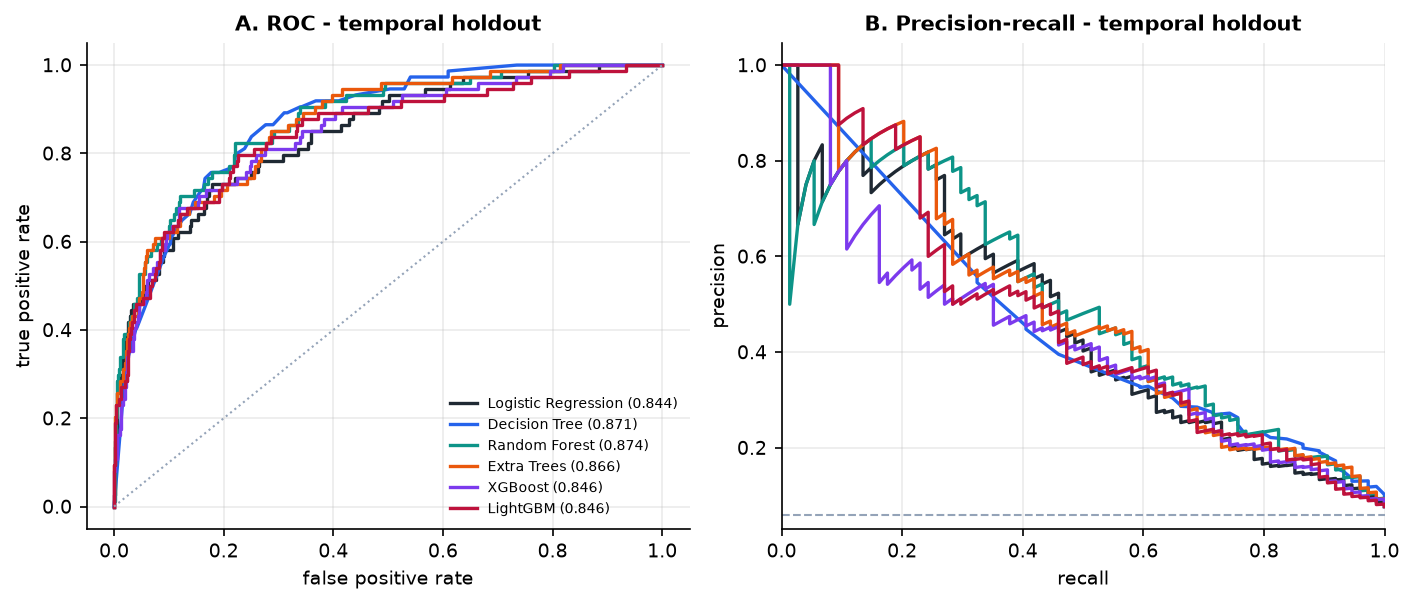
\includegraphics[width=\textwidth]{fig03_roc_pr_curves.png}
\caption{ROC curves (panel A) and precision-recall curves (panel B) on the temporal holdout.}
\label{fig:curves}
\end{figure}

\section{Calibration}

Predictions from the selected model are well calibrated, with an expected calibration error of
0.016 and a Brier score of 0.0535. A stated risk of twenty-four per cent corresponds to an
observed event frequency of approximately twenty-four per cent. This property is what makes a
threshold-based alert defensible, since a message quoting a probability must be numerically
trustworthy.

\begin{figure}[htbp]
\centering
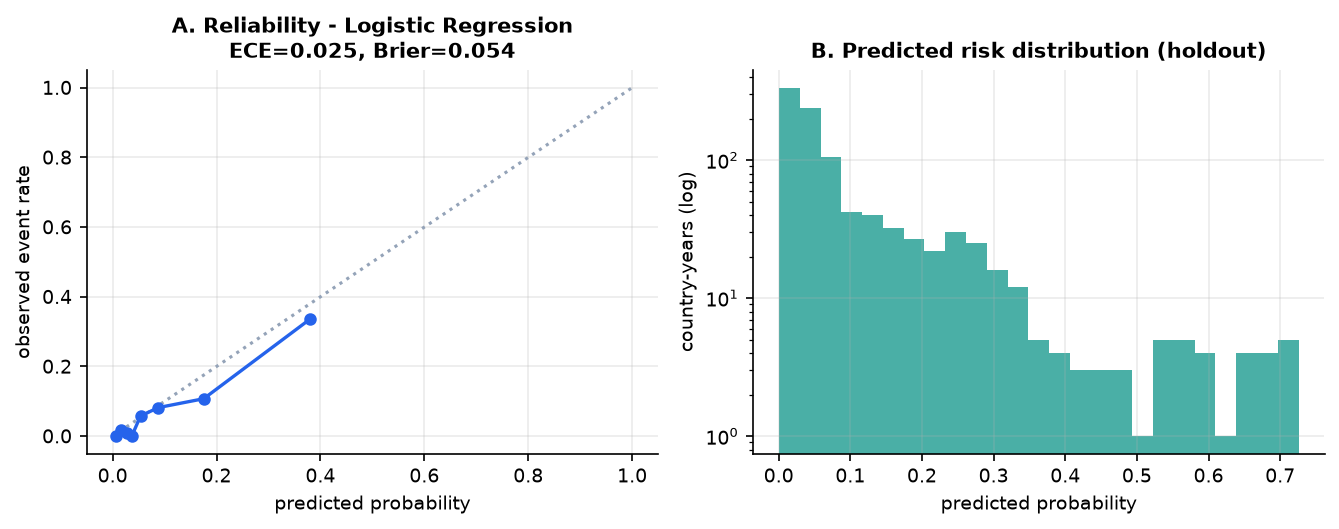
\includegraphics[width=\textwidth]{fig04_calibration.png}
\caption{Reliability diagram for the selected model on the temporal holdout, together with the
distribution of predicted risk.}
\label{fig:calib}
\end{figure}

\section{Temporal Resolution}

Aggregating observations to country and five-year period raises prevalence to 14.7\% and
improves every metric, as shown in Figure~\ref{fig:resolution}. The mechanism is that coarser
windows match the reporting cadence of the label, and a positive anywhere within the window counts
once.

\begin{figure}[htbp]
\centering
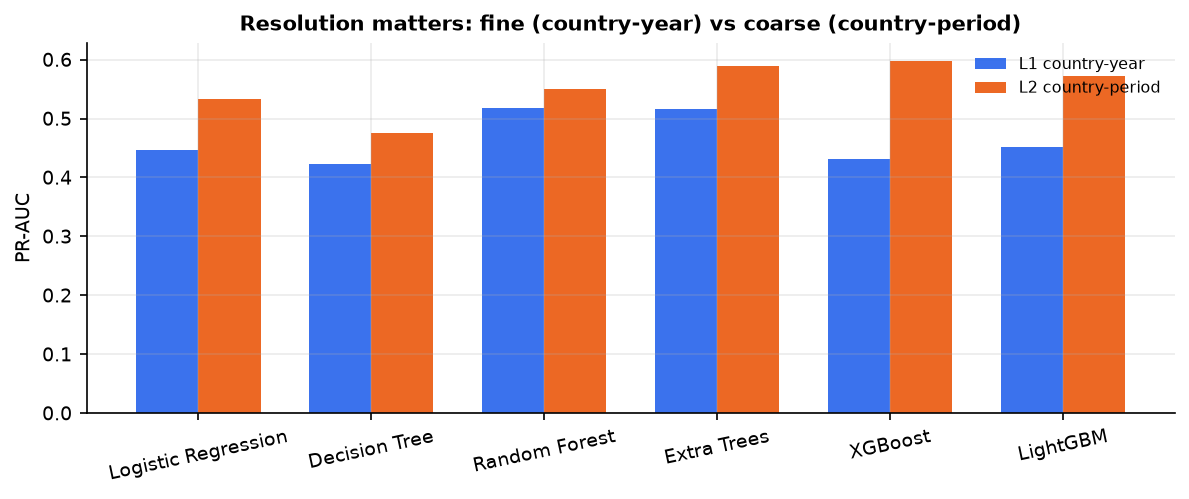
\includegraphics[width=0.85\textwidth]{fig09_resolution.png}
\caption{The same models evaluated at fine and coarse temporal resolution.}
\label{fig:resolution}
\end{figure}

\section{Ablation}
\label{sec:ablation}

Feature groups were removed and each configuration retrained, with results in
Table~\ref{tab:ablation} and Figure~\ref{fig:ablation}.

\begin{table}[htbp]
\centering
\caption{Ablation settings, using XGBoost with fixed hyperparameters.}
\label{tab:ablation}
\small
\begin{tabular}{@{}lccc@{}}
\toprule
\textbf{Feature set} & \textbf{Columns} & \textbf{PR-AUC (time)} & \textbf{PR-AUC (country)} \\
\midrule
History only & 7 & 0.407 & 0.174 \\
Population only & 14 & 0.432 & 0.241 \\
Climate only & 10 & 0.395 & 0.078 \\
Socio-geography only & 11 & 0.469 & 0.160 \\
History and population & 21 & 0.451 & 0.321 \\
All groups & 42 & 0.487 & 0.259 \\
All groups plus surveillance proxy & 44 & 0.497 & 0.261 \\
\bottomrule
\end{tabular}
\end{table}

Two results are more informative than the headline score. First, the reduced history and
population set of 21 columns reaches 0.321 under leave-country-out validation, against
0.259 for the full 42 column set. Added covariates improve in-distribution fit and reduce
transfer, because they allow the model to fit country-specific peculiarities. Second, climate
covariates alone reach only 0.078, marginally above the 5.59\% floor, which indicates
that annual country-level climatology largely encodes latitude and therefore country identity.

A separate probe adds research-output proxies as two additional columns. It moves the
leave-country-out score by +0.001, which is weak evidence that the model is not purely
tracking publication volume, but it is not proof.

\begin{figure}[htbp]
\centering
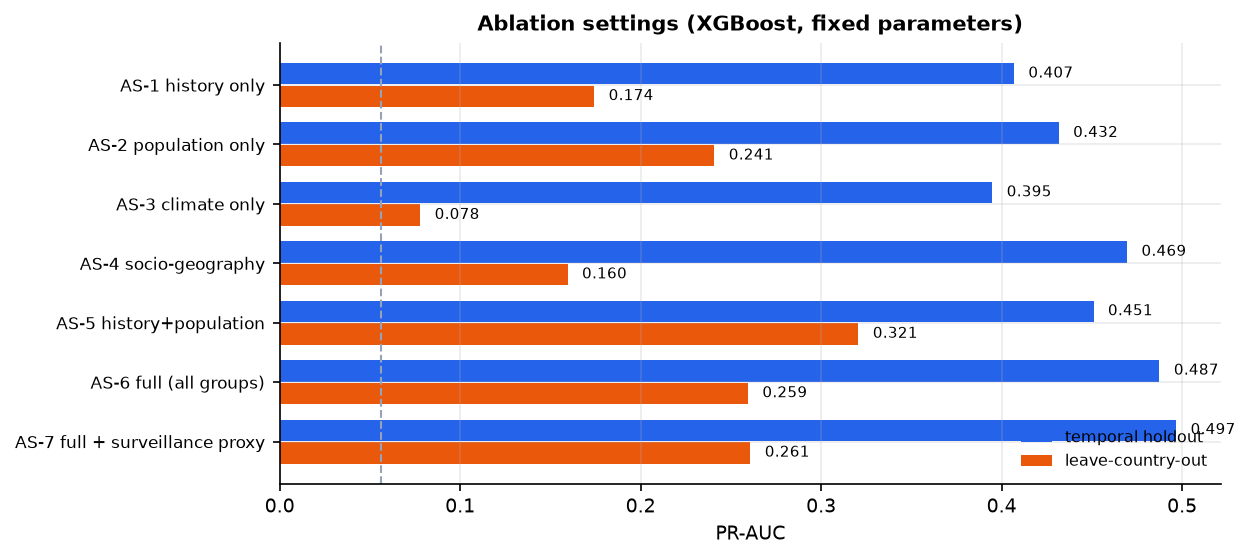
\includegraphics[width=0.92\textwidth]{fig05_ablation.png}
\caption{Ablation settings under both validation schemes.}
\label{fig:ablation}
\end{figure}

\section{Chained Pipeline}

Table~\ref{tab:chain} reports the effect of appending the stage-one population forecast to the
occurrence model.

\begin{table}[htbp]
\centering
\caption{Effect of chaining the population forecast into the occurrence model.}
\label{tab:chain}
\small
\begin{tabular}{@{}lccc@{}}
\toprule
\textbf{Variant} & \textbf{PR-AUC (time)} & \textbf{ROC-AUC (time)} & \textbf{PR-AUC (country)} \\
\midrule
Plain (no chained feature) & 0.530 & 0.854 & 0.363 \\
Chained (population forecast added) & 0.527 & 0.853 & 0.344 \\
\bottomrule
\end{tabular}
\end{table}

The population forecast performs well as a forecast, with a mean absolute error of 0.424 on the
log scale and a Spearman correlation of 0.976. The intensity stage is weaker but usable, with a
mean absolute error of 0.150 and a rank correlation of 0.465 among positive observations. The
hurdle product ranks expected annual event burden with a Spearman correlation of 0.326, and its
highest decile captures 70 of 106 observed events.

Appending the stage-one forecast to the occurrence model changes temporal PR-AUC by
-0.003, which is inside the noise band. The explanation is structural rather than a failure
of tuning. Population magnitude is already a direct feature of the occurrence model, so
forecasting it and appending the forecast supplies a less accurate copy of information the model
already holds. Chaining is expected to assist where the intermediate quantity cannot be observed
directly, which is not the case here.

This is reported as a negative result. It is a genuine finding about chained architectures for
this problem class, and it is retained rather than removed.

\section{Alert Economics}
\label{sec:alerts}

The operating characteristics of the model as a warning system are shown in
Figure~\ref{fig:alerts}. Alerting the six per cent of country-years with the highest predicted
risk captures approximately half of all observed events, and alerting twenty-eight per cent
captures eighty per cent. Uniform alerting would require full coverage for the same recall, so the
model is roughly eight times more efficient than arbitrary selection at the fifty per cent
operating point.

\begin{figure}[htbp]
\centering
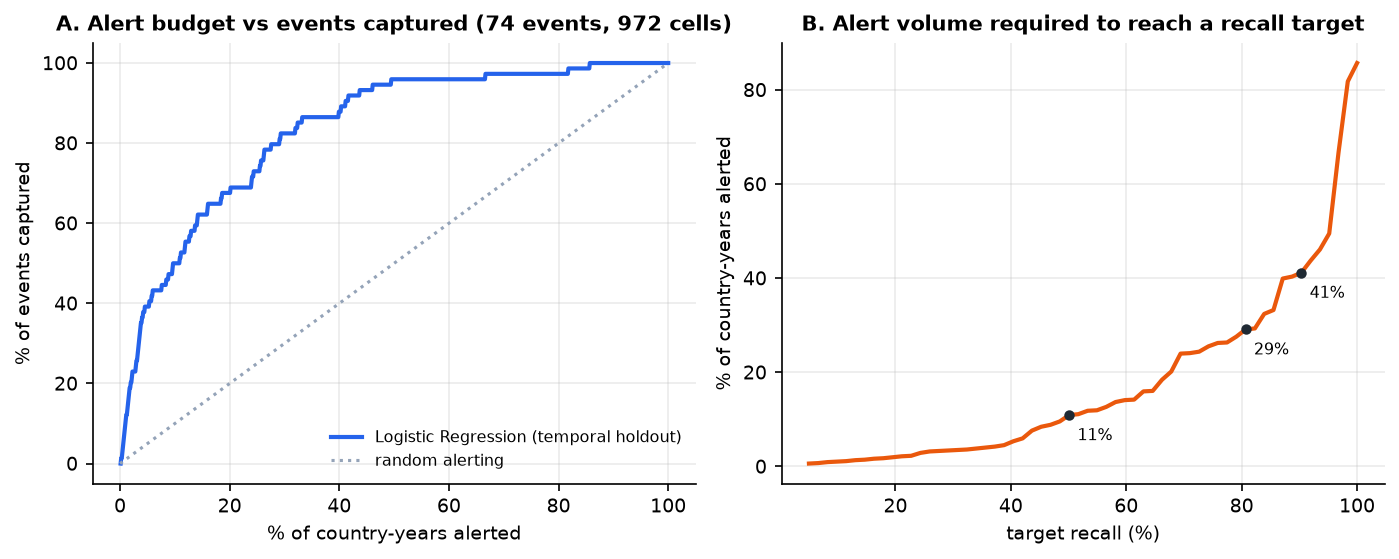
\includegraphics[width=0.92\textwidth]{fig07_alert_budget.png}
\caption{Alert economics. Panel A gives the fraction of events captured as the alert budget grows,
against random alerting. Panel B gives the alert volume required to reach a target recall.}
\label{fig:alerts}
\end{figure}

\section{Subgroup Analysis}

Table~\ref{tab:subgroup} reports leave-country-out performance by region. Skill is lowest in
Sub-Saharan Africa and in low-income countries, which are the settings in which early warning
would be most valuable. The cause is label sparsity rather than a defect in the model, since there
are few recorded events from which to learn in those strata.

\begin{table}[htbp]
\centering
\caption{Leave-country-out performance by World Bank region.}
\label{tab:subgroup}
\small
\begin{tabular}{@{}lcccc@{}}
\toprule
\textbf{Region} & \textbf{Observations} & \textbf{Events} & \textbf{ROC-AUC} & \textbf{PR-AUC} \\
\midrule
East Asia \& Pacific & 456 & 48 & 0.865 & 0.396 \\
Europe \& Central Asia & 912 & 31 & 0.826 & 0.163 \\
Latin America \& Caribbean & 551 & 12 & 0.903 & 0.381 \\
MENA, Afghanistan and Pakistan & 380 & 23 & 0.834 & 0.220 \\
Sub-Saharan Africa & 665 & 27 & 0.699 & 0.073 \\
\bottomrule
\end{tabular}
\end{table}

\begin{figure}[htbp]
\centering
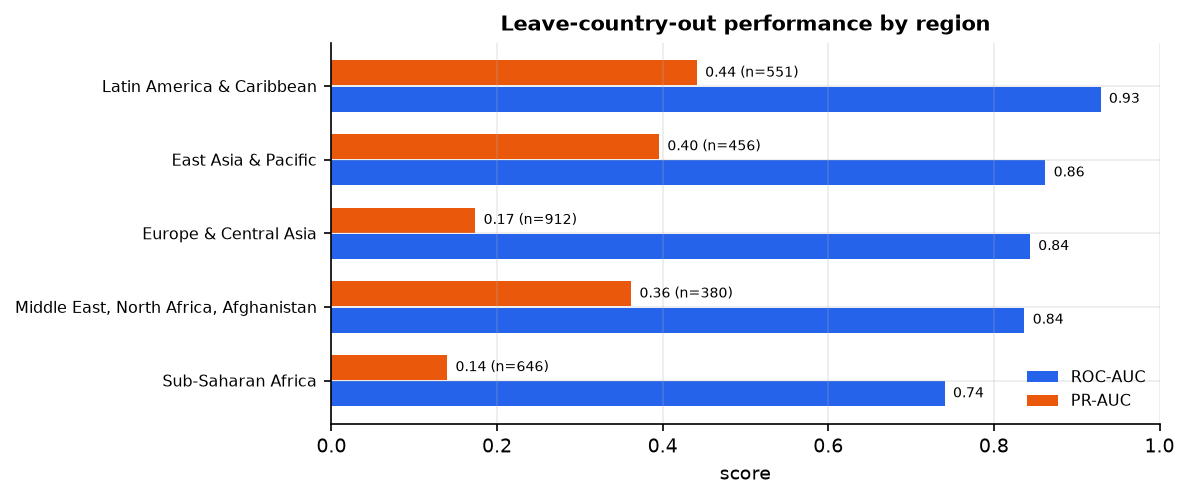
\includegraphics[width=0.9\textwidth]{fig08_subgroups.png}
\caption{Regional performance under leave-country-out validation.}
\label{fig:subgroups}
\end{figure}

\section{Discussion}

The results support four conclusions.

The model has genuine predictive skill. A precision-recall AUC of 0.554 against a base rate of
5.59\% is not explainable by chance, it survives a strictly forward-looking temporal split,
and the probabilities are calibrated to within two percentage points.

The skill does not transfer intact. Leave-country-out performance is roughly forty per cent lower
in relative terms, and this is the correct figure for planning. Any deployment to a new country
should be preceded by local validation.

The principal signal is surveillance rather than biology. The evidence is consistent across three
independent analyses: the highest-ranked features are population and connectivity measures, the
label concentrates in countries with reference laboratories, and the best-scoring cells are India,
the United States and Australia. Climate, which the original project proposal treated as a
primary input, transfers poorly at this resolution.

Simpler models transfer better. The reduced feature set outperforms the full set across countries,
and the linear baseline degrades least in absolute terms. This is a practical argument for
parsimony when positive examples are limited.

% =====================================================================
\chapter{Conclusion and Future Work}
\label{ch:concl}
% =====================================================================

\section{Conclusion}

This project set out to determine whether population-level glanders risk could be predicted from
publicly available data. Four sources that had not previously been applied to the disease were
assembled into a country-year panel covering 162 equine-holding countries, and six model families
were trained and evaluated under three validation schemes, together with a three-stage chained
pipeline.

The central finding is that prediction is possible, and that the achievable performance is
moderate. On a strictly forward-looking temporal holdout the strongest model reaches a
precision-recall AUC of 0.554 against a base rate of 5.59\%, an approximately 10-fold
lift, with an expected calibration error of 0.016. Used as a warning system, it captures half of
all observed events while alerting six per cent of country-years.

The second finding is that the skill is fragile across geography. Leave-country-out performance is
approximately forty per cent lower in relative terms, and the decline is concentrated in the
regions where early warning would be most useful.

The third finding concerns what the model is learning. Three independent analyses
converge on the same conclusion. The highest-ranked features are population size and reporting
capacity rather than biological drivers. The label concentrates in countries that operate
reference laboratories. And the highest-scoring cells are the countries with the strongest
veterinary publishing record. The model predicts where glanders will be documented, which is
useful for directing surveillance, and it is not a map of where the organism is present.

The fourth finding is negative. The chained design specified in the project proposal does not
improve discrimination, because the intermediate quantity is already available as a direct
feature. This is reported rather than omitted, since it is a reproducible result about chained
architectures for this problem class.

\section{Future Work}

Four directions follow directly from the limitations identified in this report.

\textbf{Modelling reporting effort explicitly.} The most important extension is to treat
surveillance capacity as a modelled quantity rather than an incidental covariate. This could be
done by using publication volume as a separate offset, or by fitting a two-part model in which
detection and occurrence are estimated jointly. Without this, gains in predictive score are
likely to reflect reporting practice rather than disease.

\textbf{Validating the label extractor.} The 263 extracted events have not been checked against a
hand-annotated reference set. Annotating a stratified sample of several hundred abstracts would
allow precision and recall of the extractor itself to be reported, and would bound the label noise
that currently propagates into every downstream estimate.

\textbf{District-level modelling for India.} The original proposal envisaged district-month
resolution for India, where the disease is concentrated in a small number of states. Public
district-level covariates for equine population and climate would need to be assembled, but the
resolution would match the scale at which control measures are applied.

\textbf{Operational calibration under drift.} A deployed model requires periodic recalibration as
reporting practice changes. The calibration framework used here is a single point estimate; a
production system would need drift monitoring and a defined retraining trigger.

Two smaller extensions are worth noting. Incorporating WOAH WAHIS official outbreak records as a
second label source would allow the literature-derived label to be validated where the two
overlap. And a cost-sensitive threshold, in which the relative cost of a missed outbreak and a
false alert is stated explicitly, would replace the F1-optimal threshold used here with one
matched to the programme's actual priorities.

% ============================== REFERENCES ==============================
\newpage
\chapter*{Bibliography}
\addcontentsline{toc}{chapter}{Bibliography}
\renewcommand{\bibname}{}
\begin{multicols}{2}
\begin{thebibliography}{99}
\footnotesize
\setlength{\itemsep}{0.15em}
\setlength{\parskip}{0pt}
\bibitem{khan2013} Khan I, Wieler LH, Melzer F, et al. Glanders in animals: a review on epidemiology, clinical presentation, diagnosis and countermeasures. \emph{Transboundary and Emerging Diseases}. 2013. doi:10.1111/j.1865-1682.2012.01342.x
\bibitem{kanani2026} Kanani Y, Oryan A, Derakhshandeh A. Glanders: past, present and future of a neglected zoonosis as a threat in veterinary and human health. \emph{Veterinary Medicine and Science}. 2026. doi:10.1002/vms3.70950
\bibitem{purnama2026} Purnama MTE, Firdausy LW, Fikri F, et al. Seroprevalence and associated epidemiological drivers of glanders in horses: a systematic review and meta-analysis. \emph{Research in Veterinary Science}. 2026;106416. doi:10.1016/j.rvsc.2026.106416
\bibitem{mota2022} Mota RA, Pinheiro J\'unior JW. Current status of glanders in Brazil: recent advances and challenges. \emph{Brazilian Journal of Microbiology}. 2022. doi:10.1007/s42770-022-00814-1
\bibitem{singha2026} Singha H, Shanmugasundaram K, Jhandai P, et al. Surveillance of equine glanders in India (2019--2023): prevalence estimate, risk analysis and future strategy. \emph{Microbial Pathogenesis}. 2026;217:108597. doi:10.1016/j.micpath.2026.108597
\bibitem{singha2020} Singha H, Shanmugasundaram K, Tripathi BN, et al. Serological surveillance and clinical investigation of glanders among indigenous equines in India from 2015 to 2018. \emph{Transboundary and Emerging Diseases}. 2020. doi:10.1111/tbed.13475
\bibitem{malik2012} Malik P, Singha H, Khurana SK, et al. Emergence and re-emergence of glanders in India: a description of outbreaks from 2006 to 2011. \emph{Veterinaria Italiana}. 2012. PMID:22718333
\bibitem{fonseca2019} Fonseca-Rodr\'iguez O, Pinheiro J\'unior JW, Mota RA. Spatiotemporal analysis of glanders in Brazil. \emph{Journal of Equine Veterinary Science}. 2019. doi:10.1016/j.jevs.2019.03.216
\bibitem{hollings2017} Hollings T, Robinson A, van Andel M, et al. Species distribution models: a comparison of statistical approaches for livestock and disease epidemics. \emph{PLOS ONE}. 2017;12(8):e0183626. doi:10.1371/journal.pone.0183626
\bibitem{alshatti2026} Alshatti M, Al-Hemoud A, Othman A, et al. A risk prediction model for highly pathogenic avian influenza outbreaks in Kuwait. \emph{Frontiers in Veterinary Science}. 2026. doi:10.3389/fvets.2026.1843962
\bibitem{kane2014} Kane MJ, Price N, Scotch M, Rabinowitz P. Comparison of ARIMA and Random Forest time series models for prediction of avian influenza H5N1 outbreaks. \emph{BMC Bioinformatics}. 2014;15:276. doi:10.1186/1471-2105-15-276
\bibitem{walsh2019} Walsh DP, Ma TF, Ip HS, Zhu J. Artificial intelligence and avian influenza: using machine learning to enhance active surveillance for avian influenza viruses. \emph{Transboundary and Emerging Diseases}. 2019. doi:10.1111/tbed.13318
\bibitem{yoo2022} Yoo DS, Song YH, Choi DW, et al. Machine learning-driven dynamic risk prediction for highly pathogenic avian influenza at poultry farms in the Republic of Korea. \emph{Transboundary and Emerging Diseases}. 2021. doi:10.1111/tbed.14419
\bibitem{moawad2019} Moawad AA, Silge A, Bocklitz T, Fischer K, R\"osch P, Roesler U, Elschner MC, Popp J, Neubauer H. A machine learning-based Raman spectroscopic assay for the identification of \emph{Burkholderia mallei} and related species. \emph{Molecules}. 2019;24(24):4516. doi:10.3390/molecules24244516
\bibitem{stoeckel2015} St\"ockel S, Meisel S, Elschner M, Melzer F, R\"osch P, Popp J. Raman spectroscopic detection and identification of \emph{Burkholderia mallei} and \emph{Burkholderia pseudomallei}. \emph{Analytical and Bioanalytical Chemistry}. 2015;407(3):833--843. doi:10.1007/s00216-014-7906-5
\bibitem{collier2012} Collier N. Uncovering text mining: a survey of current work on web-based epidemic intelligence. \emph{Global Public Health}. 2012. doi:10.1080/17441692.2012.699975
\bibitem{lejeune2015} Lejeune G, Brixtel R, Doucet A, et al. Multilingual event extraction for epidemic detection. \emph{Artificial Intelligence in Medicine}. 2015. doi:10.1016/j.artmed.2015.06.005
\bibitem{chen2016} Chen T, Guestrin C. XGBoost: a scalable tree boosting system. In: \emph{Proceedings of the 22nd ACM SIGKDD International Conference on Knowledge Discovery and Data Mining}. 2016:785--794. doi:10.1145/2939672.2939785
\bibitem{ke2017} Ke G, Meng Q, Finley T, et al. LightGBM: a highly efficient gradient boosting decision tree. In: \emph{Advances in Neural Information Processing Systems 30 (NIPS)}. 2017:3146--3154.
\bibitem{breiman2001} Breiman L. Random forests. \emph{Machine Learning}. 2001. doi:10.1023/A:1010933404324
\bibitem{lundberg2017} Lundberg SM, Lee SI. A unified approach to interpreting model predictions. In: \emph{Advances in Neural Information Processing Systems 30 (NIPS)}. 2017:4765--4774. arXiv:1705.07874
\bibitem{saito2015} Saito T, Rehmsmeier M. The precision-recall plot is more informative than the ROC plot when evaluating binary classifiers on imbalanced datasets. \emph{PLOS ONE}. 2015;10(3):e0118432. doi:10.1371/journal.pone.0118432
\bibitem{davis2006} Davis J, Goadrich M. The relationship between precision-recall and ROC curves. In: \emph{Proceedings of the 23rd International Conference on Machine Learning}. 2006:233--240. doi:10.1145/1143844.1143874
\bibitem{roberts2017} Roberts DR, Bahn V, Ciuti S, et al. Cross-validation strategies for data with temporal, spatial, hierarchical, or phylogenetic structure. \emph{Ecography}. 2017. doi:10.1111/ecog.02881
\bibitem{niculescu2005} Niculescu-Mizil A, Caruana R. Predicting good probabilities with supervised learning. In: \emph{Proceedings of the 22nd International Conference on Machine Learning}. 2005:625--632. doi:10.1145/1102351.1102430
\bibitem{huang2020} Huang Y, Li W, Macheret F, et al. A tutorial on calibration measurements and calibration models for clinical prediction models. \emph{Journal of the American Medical Informatics Association}. 2020;27(4):621--633. doi:10.1093/jamia/ocz228
\bibitem{wahis} WOAH. World Animal Health Information System (WAHIS). \url{https://wahis.woah.org}
\bibitem{dahd2025} Department of Animal Husbandry and Dairying, Government of India. \emph{National Action Plan for Control and Eradication of Glanders in India} (Revised 2025). New Delhi: DAHD; 2025.
\bibitem{faostat} FAO. FAOSTAT: crops and livestock products. \url{https://www.fao.org/faostat}
\bibitem{power} NASA Langley Research Center. POWER agroclimatology API. \url{https://power.larc.nasa.gov}
\bibitem{wdi} World Bank. World Development Indicators. \url{https://databank.worldbank.org}
\bibitem{europepmc} Europe PMC literature search API. \url{https://europepmc.org}
\end{thebibliography}
\end{multicols}


\end{document}
